\documentclass{beamer}
\usepackage{../../shared/styles/custom}
\usepackage{../../shared/styles/conventions}

\usepackage{amsfonts}
\def\checkmark{\tikz\fill[scale=0.4](0,.35) -- (.25,0) -- (1,.7) -- (.25,.15) -- cycle;} 
%\beamerdefaultoverlayspecification{<+->}
% \newcommand{\data}{\mathcal{D}}
% \newcommand\Item[1][]{%
% 	\ifx\relax#1\relax  \item \else \item[#1] \fi
% 	\abovedisplayskip=0pt\abovedisplayshortskip=0pt~\vspace*{-\baselineskip}}



\graphicspath{ {./SVM/} }

\title{Support Vector Machines}
\date{\today}
\author{Nipun Batra}
\institute{IIT Gandhinagar}
\begin{document}
	\maketitle
	
	\begin{frame}{Non-Linearly Separable Data}
	\begin{minipage}{0.3\textwidth}
    % Show the image at item three and afterwards
    
      \begin{figure}
      
        % From https://i.imgur.com/AyzVOIO.jpg
       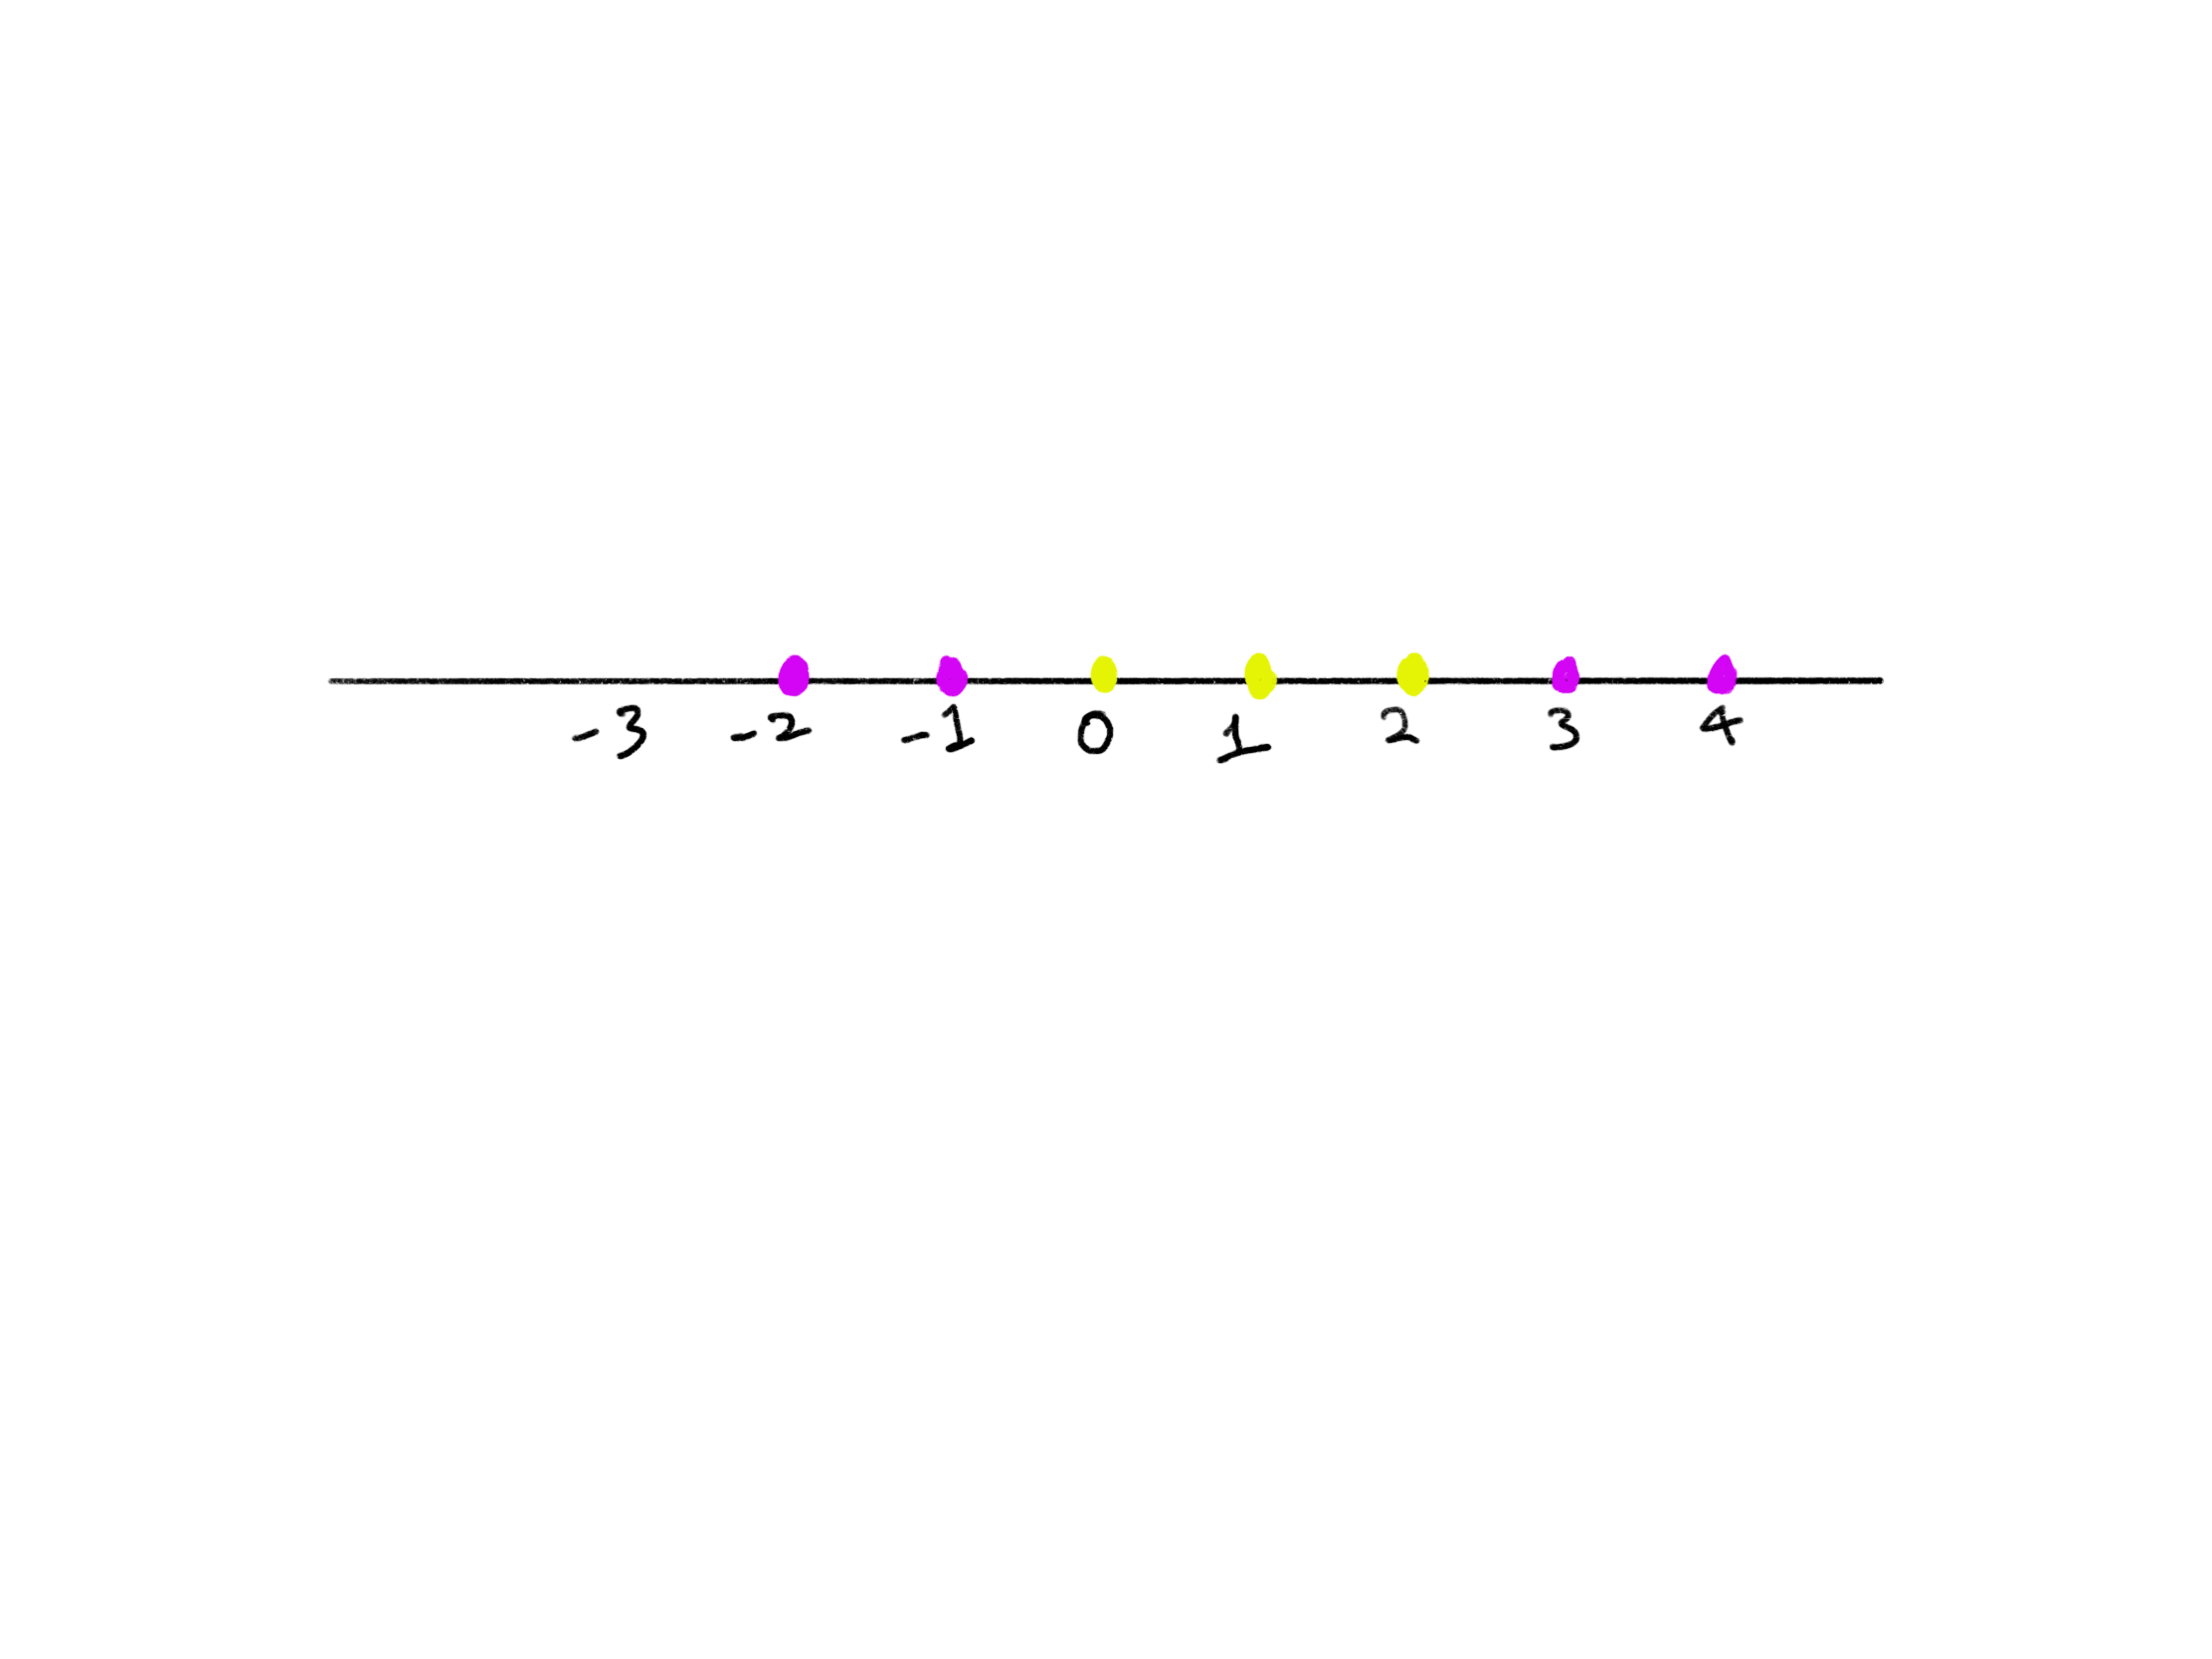
\includegraphics[height=2.5\textwidth]{pik1.png}
      \end{figure}
  \end{minipage} \\
  \vspace{-3cm}
	    Data not separate in $\mathbb{R}$ \\
	    Can we still use SVM? \\
	    Yes!\\
	    How? Project data to a higher dimensional space.
	\end{frame}
	\begin{frame}{Non-Lineary Separable Data}
	\vspace{-1cm}
	    \begin{figure}
        % From https://i.imgur.com/AyzVOIO.jpg
       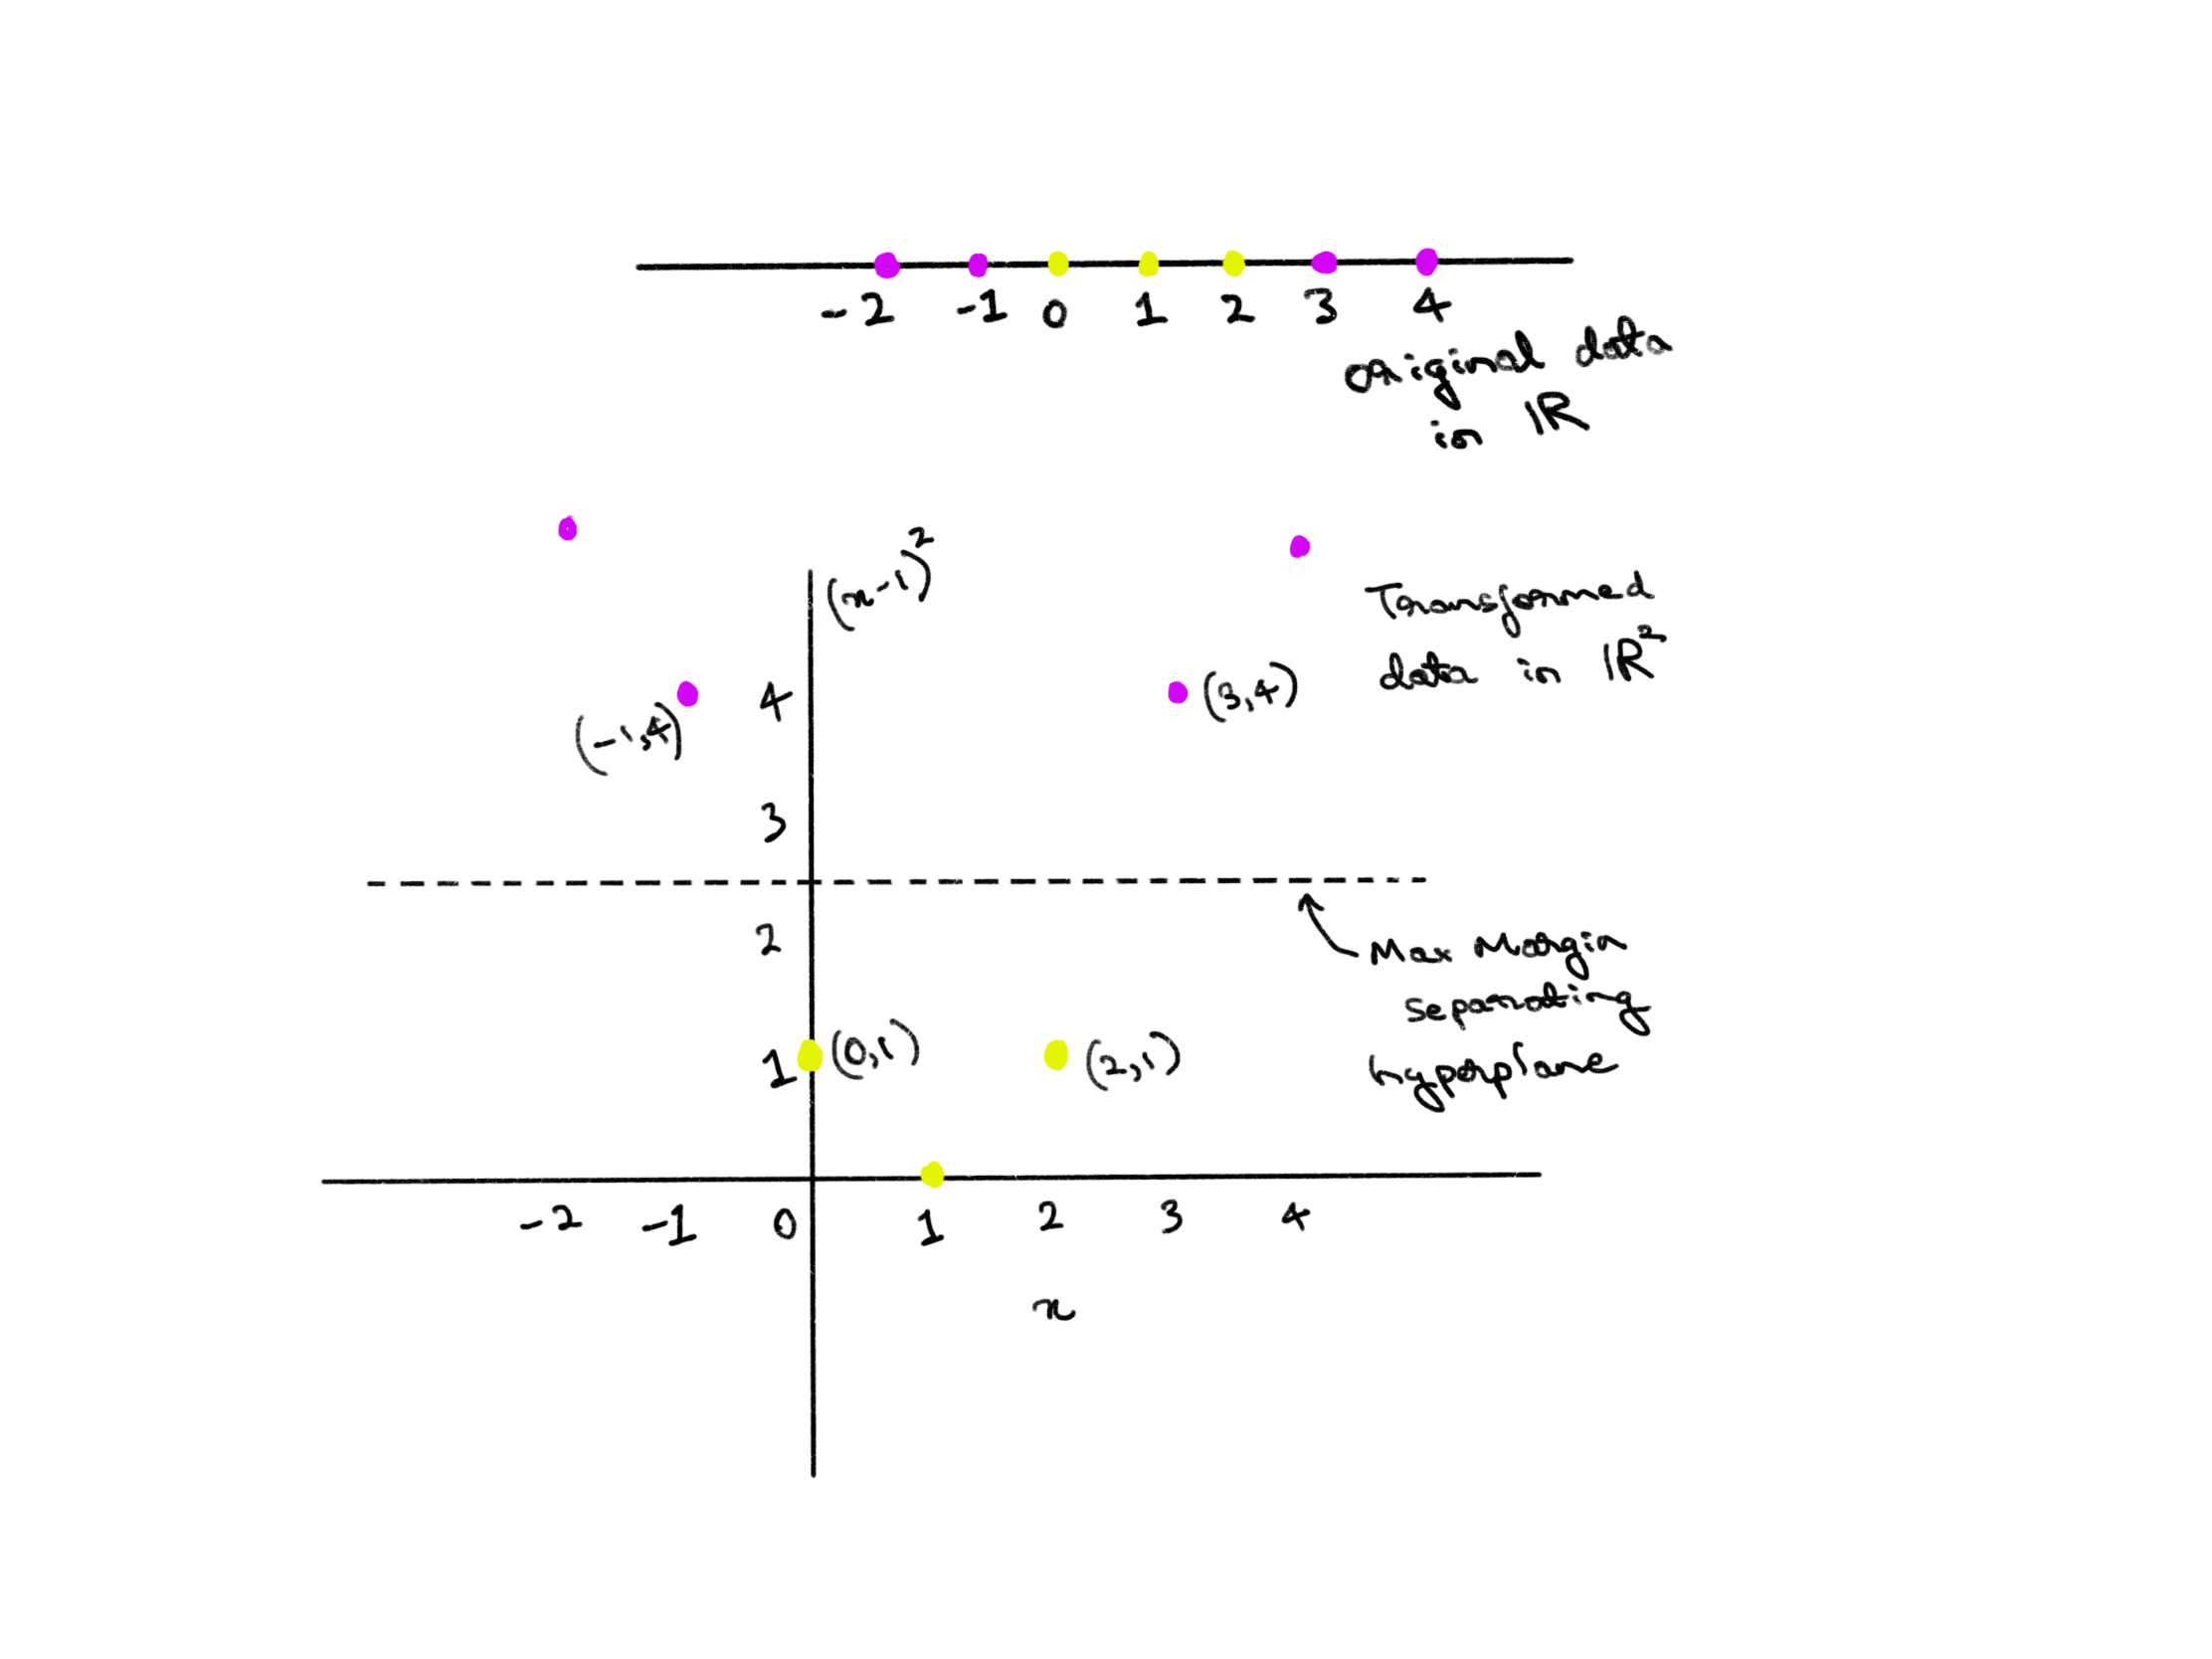
\includegraphics[height=0.8\textwidth]{pik2.png}
      \end{figure}
	\end{frame}
	\begin{frame}{Non-Lineary Separable Data}
	\vspace{-0.5cm}
	    \begin{figure}
        % From https://i.imgur.com/AyzVOIO.jpg
       \hspace{-1cm}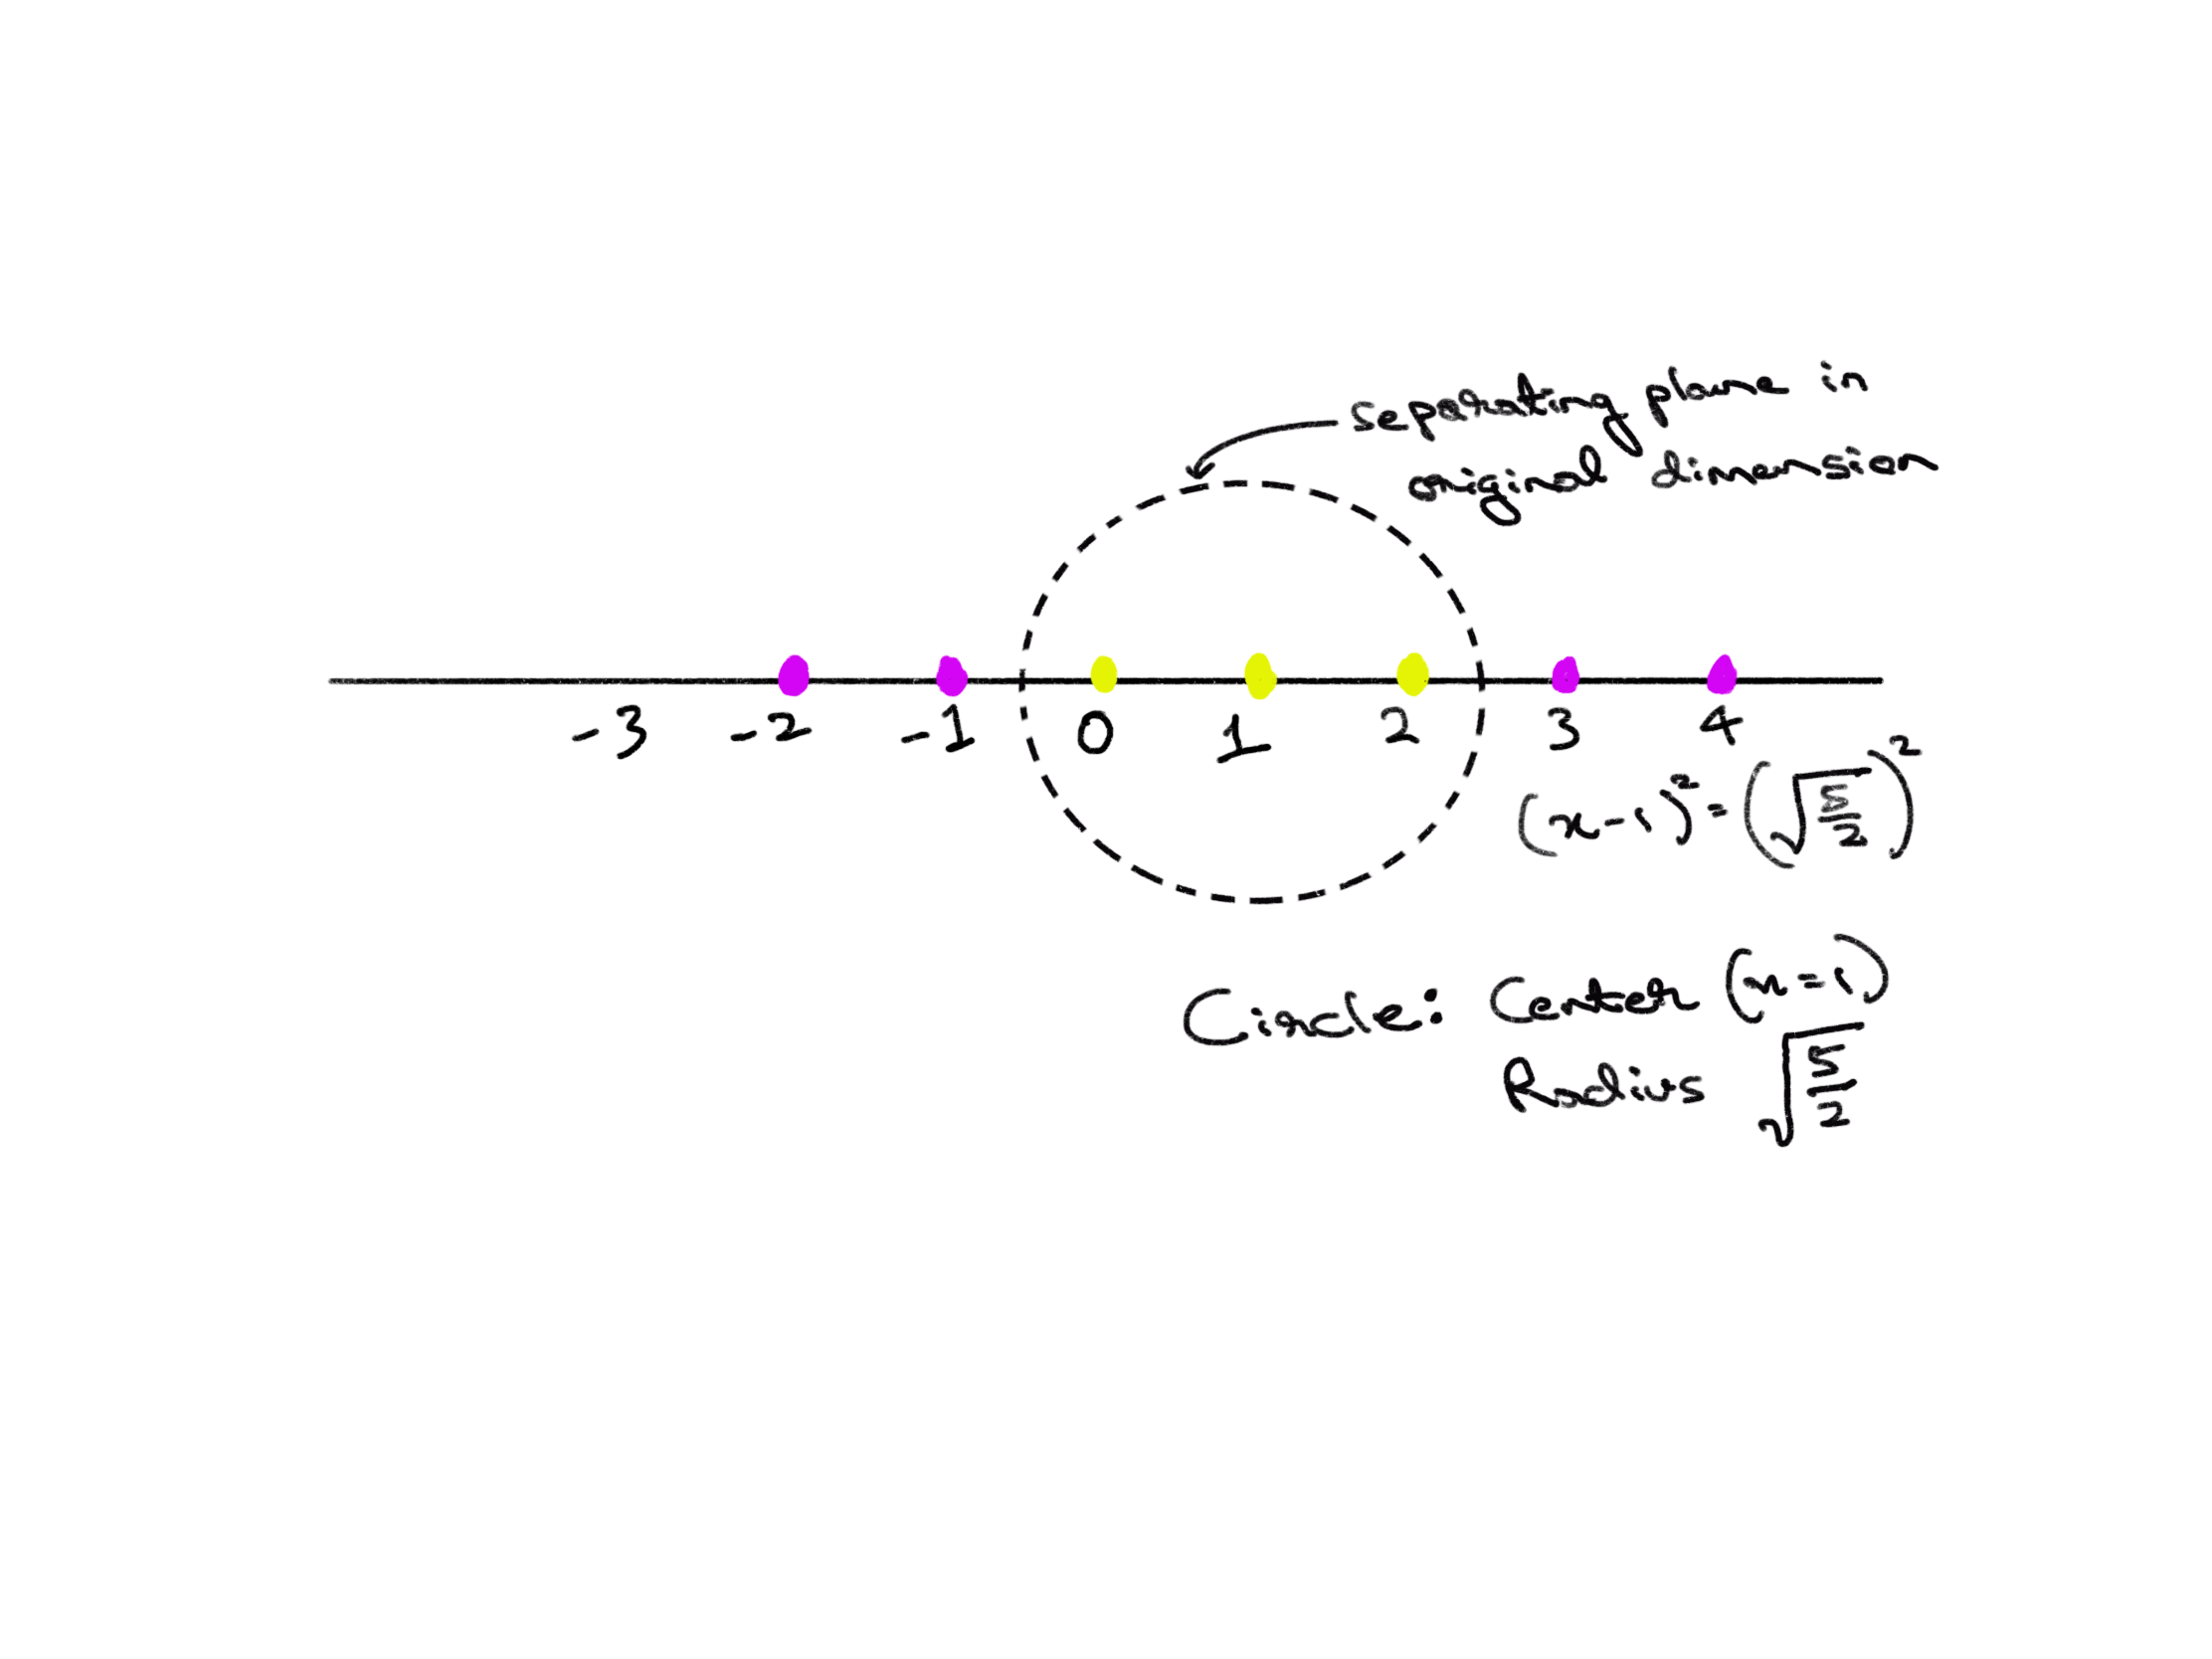
\includegraphics[height=0.8\textwidth]{pik3.png}
      \end{figure}
	\end{frame}
	\begin{frame}{Another Example Transformation}
	    \begin{figure}
        % From https://i.imgur.com/AyzVOIO.jpg
       \hspace{-1cm}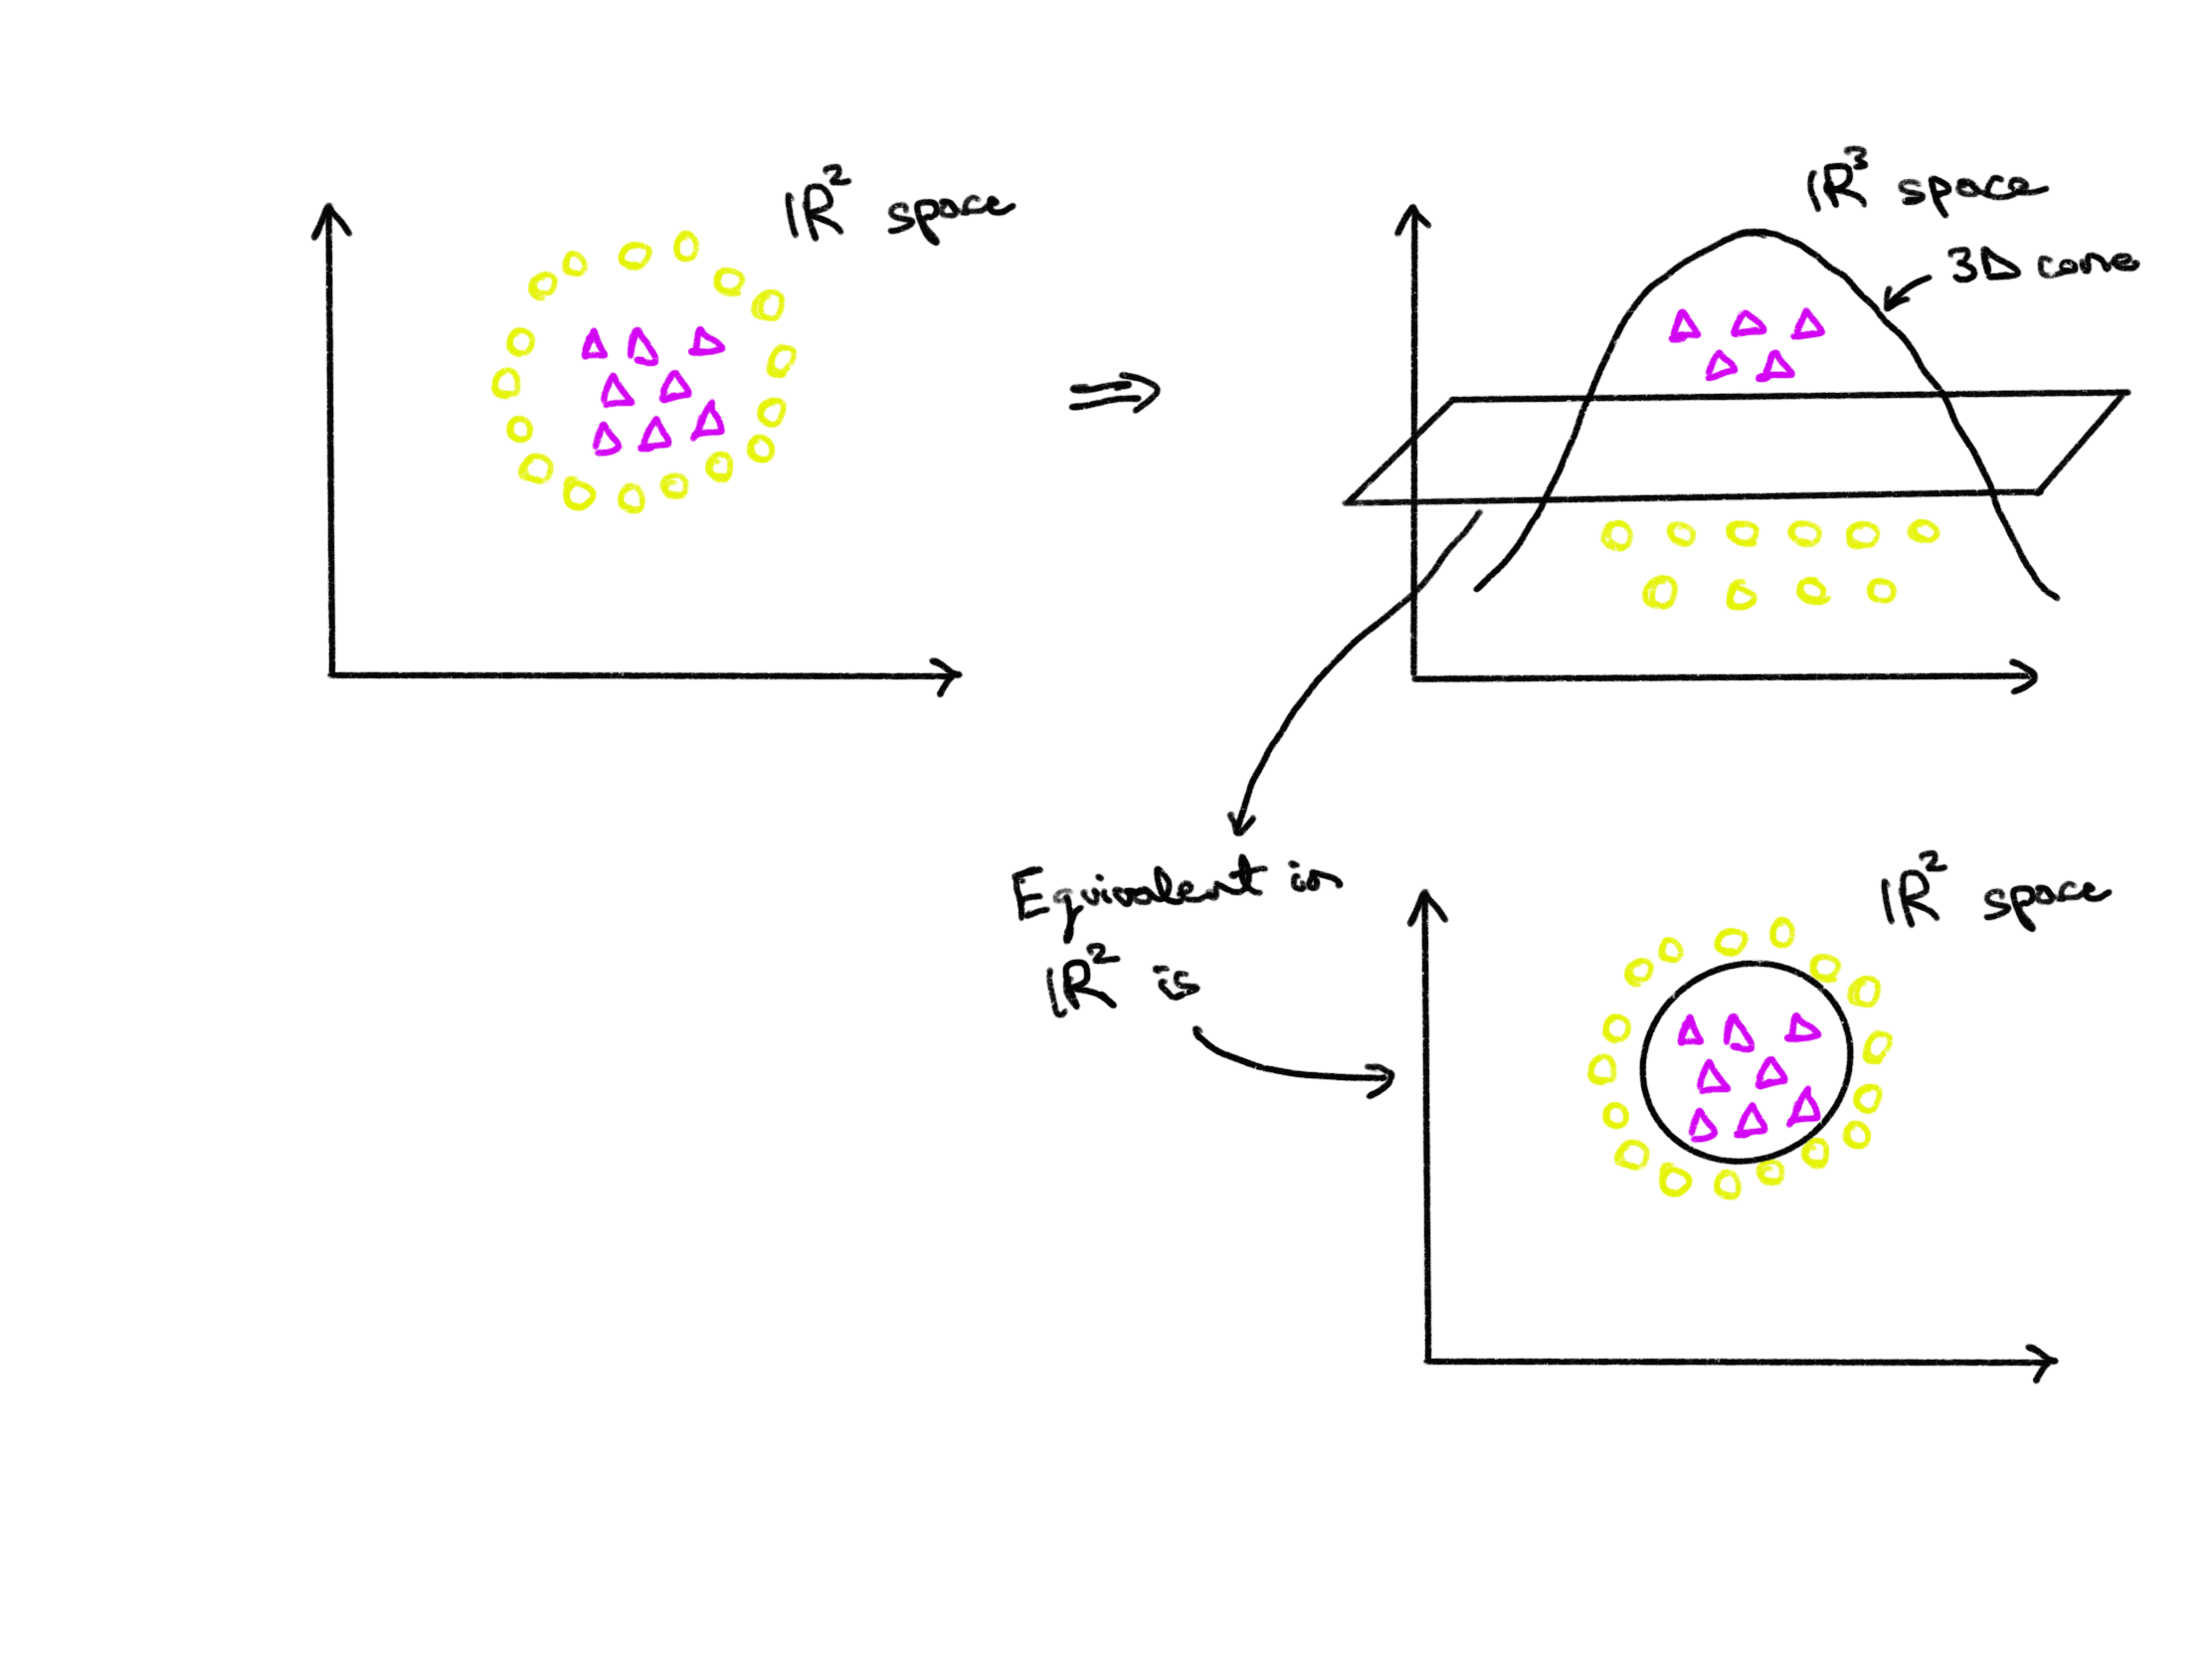
\includegraphics[height=0.8\textwidth]{pik4.png}
      \end{figure}
	\end{frame}
	\begin{frame}{Projection/Transformation Function}
	        $\phi : \mathbb{R}^{d} \rightarrow \mathbb{R}^{D}$
	    
	    where, $d$ = original dimension \\
	    \hspace{1cm} $D$ = new dimension \\
	    In our example:\\
	    \hspace{1cm} $d = 1; D = 2$ 
	\end{frame}
	\begin{frame}{}
	    Linear SVM:\\
	    \hspace{1cm} Maximize\\
	    \begin{equation*}
	        L(\alpha) = \sum_{i=1}^{N}\alpha_{i} - \frac{1}{2}\sum_{i=1}^{N}\sum_{j=1}^{N}\alpha_{i}\alpha_{j}y_{i}y_{j}\overline{x_{i}}.\overline{x_{j}}
	    \end{equation*}
	    \hspace{1cm} such that constriants are satisfied.\\
	   \hspace{5cm} $\downarrow$\\
	   \hspace{3.8cm} Transformation ($\phi$)\\
	   \hspace{5cm} $\downarrow$\\
	   \begin{equation*}
	       L(\alpha) = \sum_{i=1}^{N}\alpha_{i} - \frac{1}{2}\sum_{i=1}^{N}\sum_{j=1}^{N}\alpha_{i}\alpha_{j}y_{i}y_{j}\phi(\overline{x_{i}}).\phi(\overline{x_{j}})
	   \end{equation*}
	\end{frame}
	\begin{frame}{Trivial Example (Again)}
	    \begin{figure}
        % From https://i.imgur.com/AyzVOIO.jpg
       \hspace{-1cm}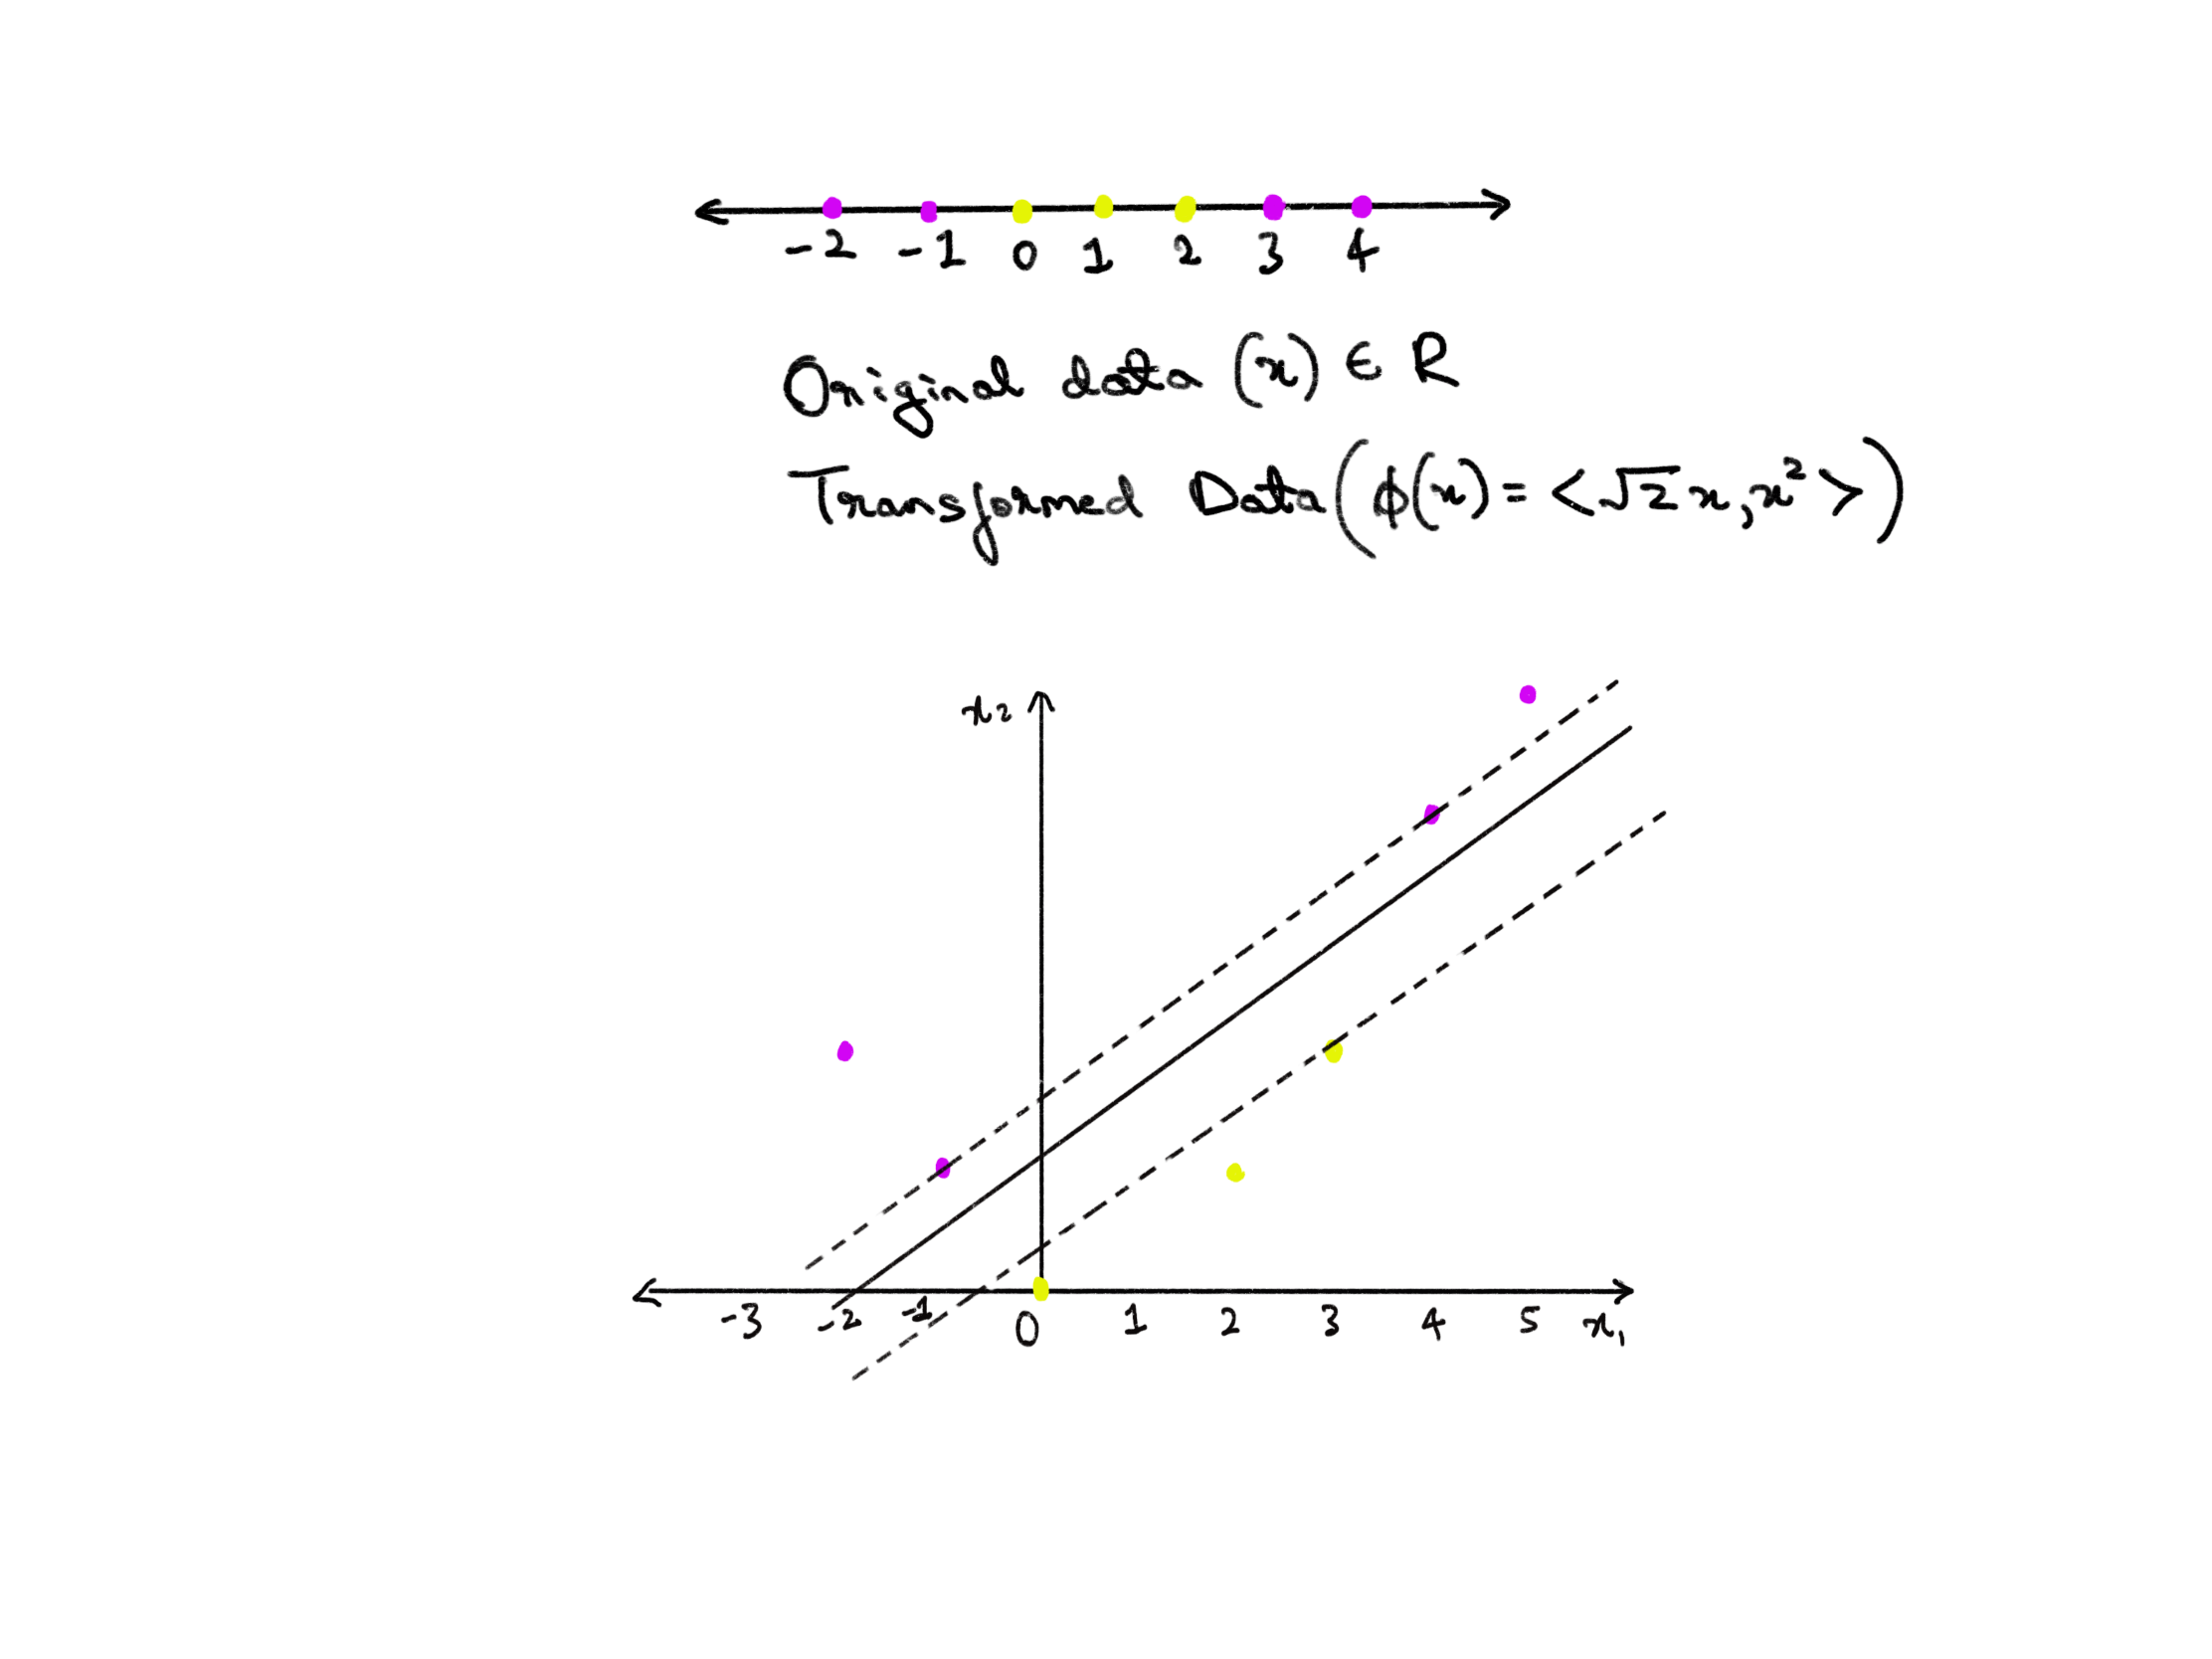
\includegraphics[height=0.8\textwidth]{pik5.png}
      \end{figure}
	\end{frame}
	\begin{frame}{Steps}
	    \begin{enumerate}
	        \item Compute $\phi(x)$ for each point \\
	        \begin{equation*}
	            \phi: \mathbb{R}^{d} \rightarrow \mathbb{R}^{D}
	        \end{equation*}
	        \item Compute dot products over $\mathbb{R}^{D}$ space
	    \end{enumerate}
	    \hspace{0.1cm} Q. If $D >> d$ \\
	    \hspace{0.6cm} Both steps are expensive!
	\end{frame}
	\begin{frame}{Kernel Trick}
	
	    Can we compute K($\bar{x}_{i}, \bar{x}_{j})$ \\
	    s.t. \\
	    K($\bar{x}_{i}, \bar{x}_{j}) = \phi(\bar{x}_{i}).\phi(\bar{x}_{j})$ \\
	    where, \\
	    K($\bar{x}_{i}, \bar{x}_{j})$ is some function of dot product in original dimension \\
	    $\phi(\bar{x}_{i}).\phi(\bar{x}_{j})$ is dot product in high dimensions (after transformation)
	\end{frame}
	\begin{frame}{Kernel Trick}
	\vspace{-2cm}
	\begin{minipage}{0.3\textwidth}
    % Show the image at item three and afterwards
    
      \begin{figure}
      
        % From https://i.imgur.com/AyzVOIO.jpg
       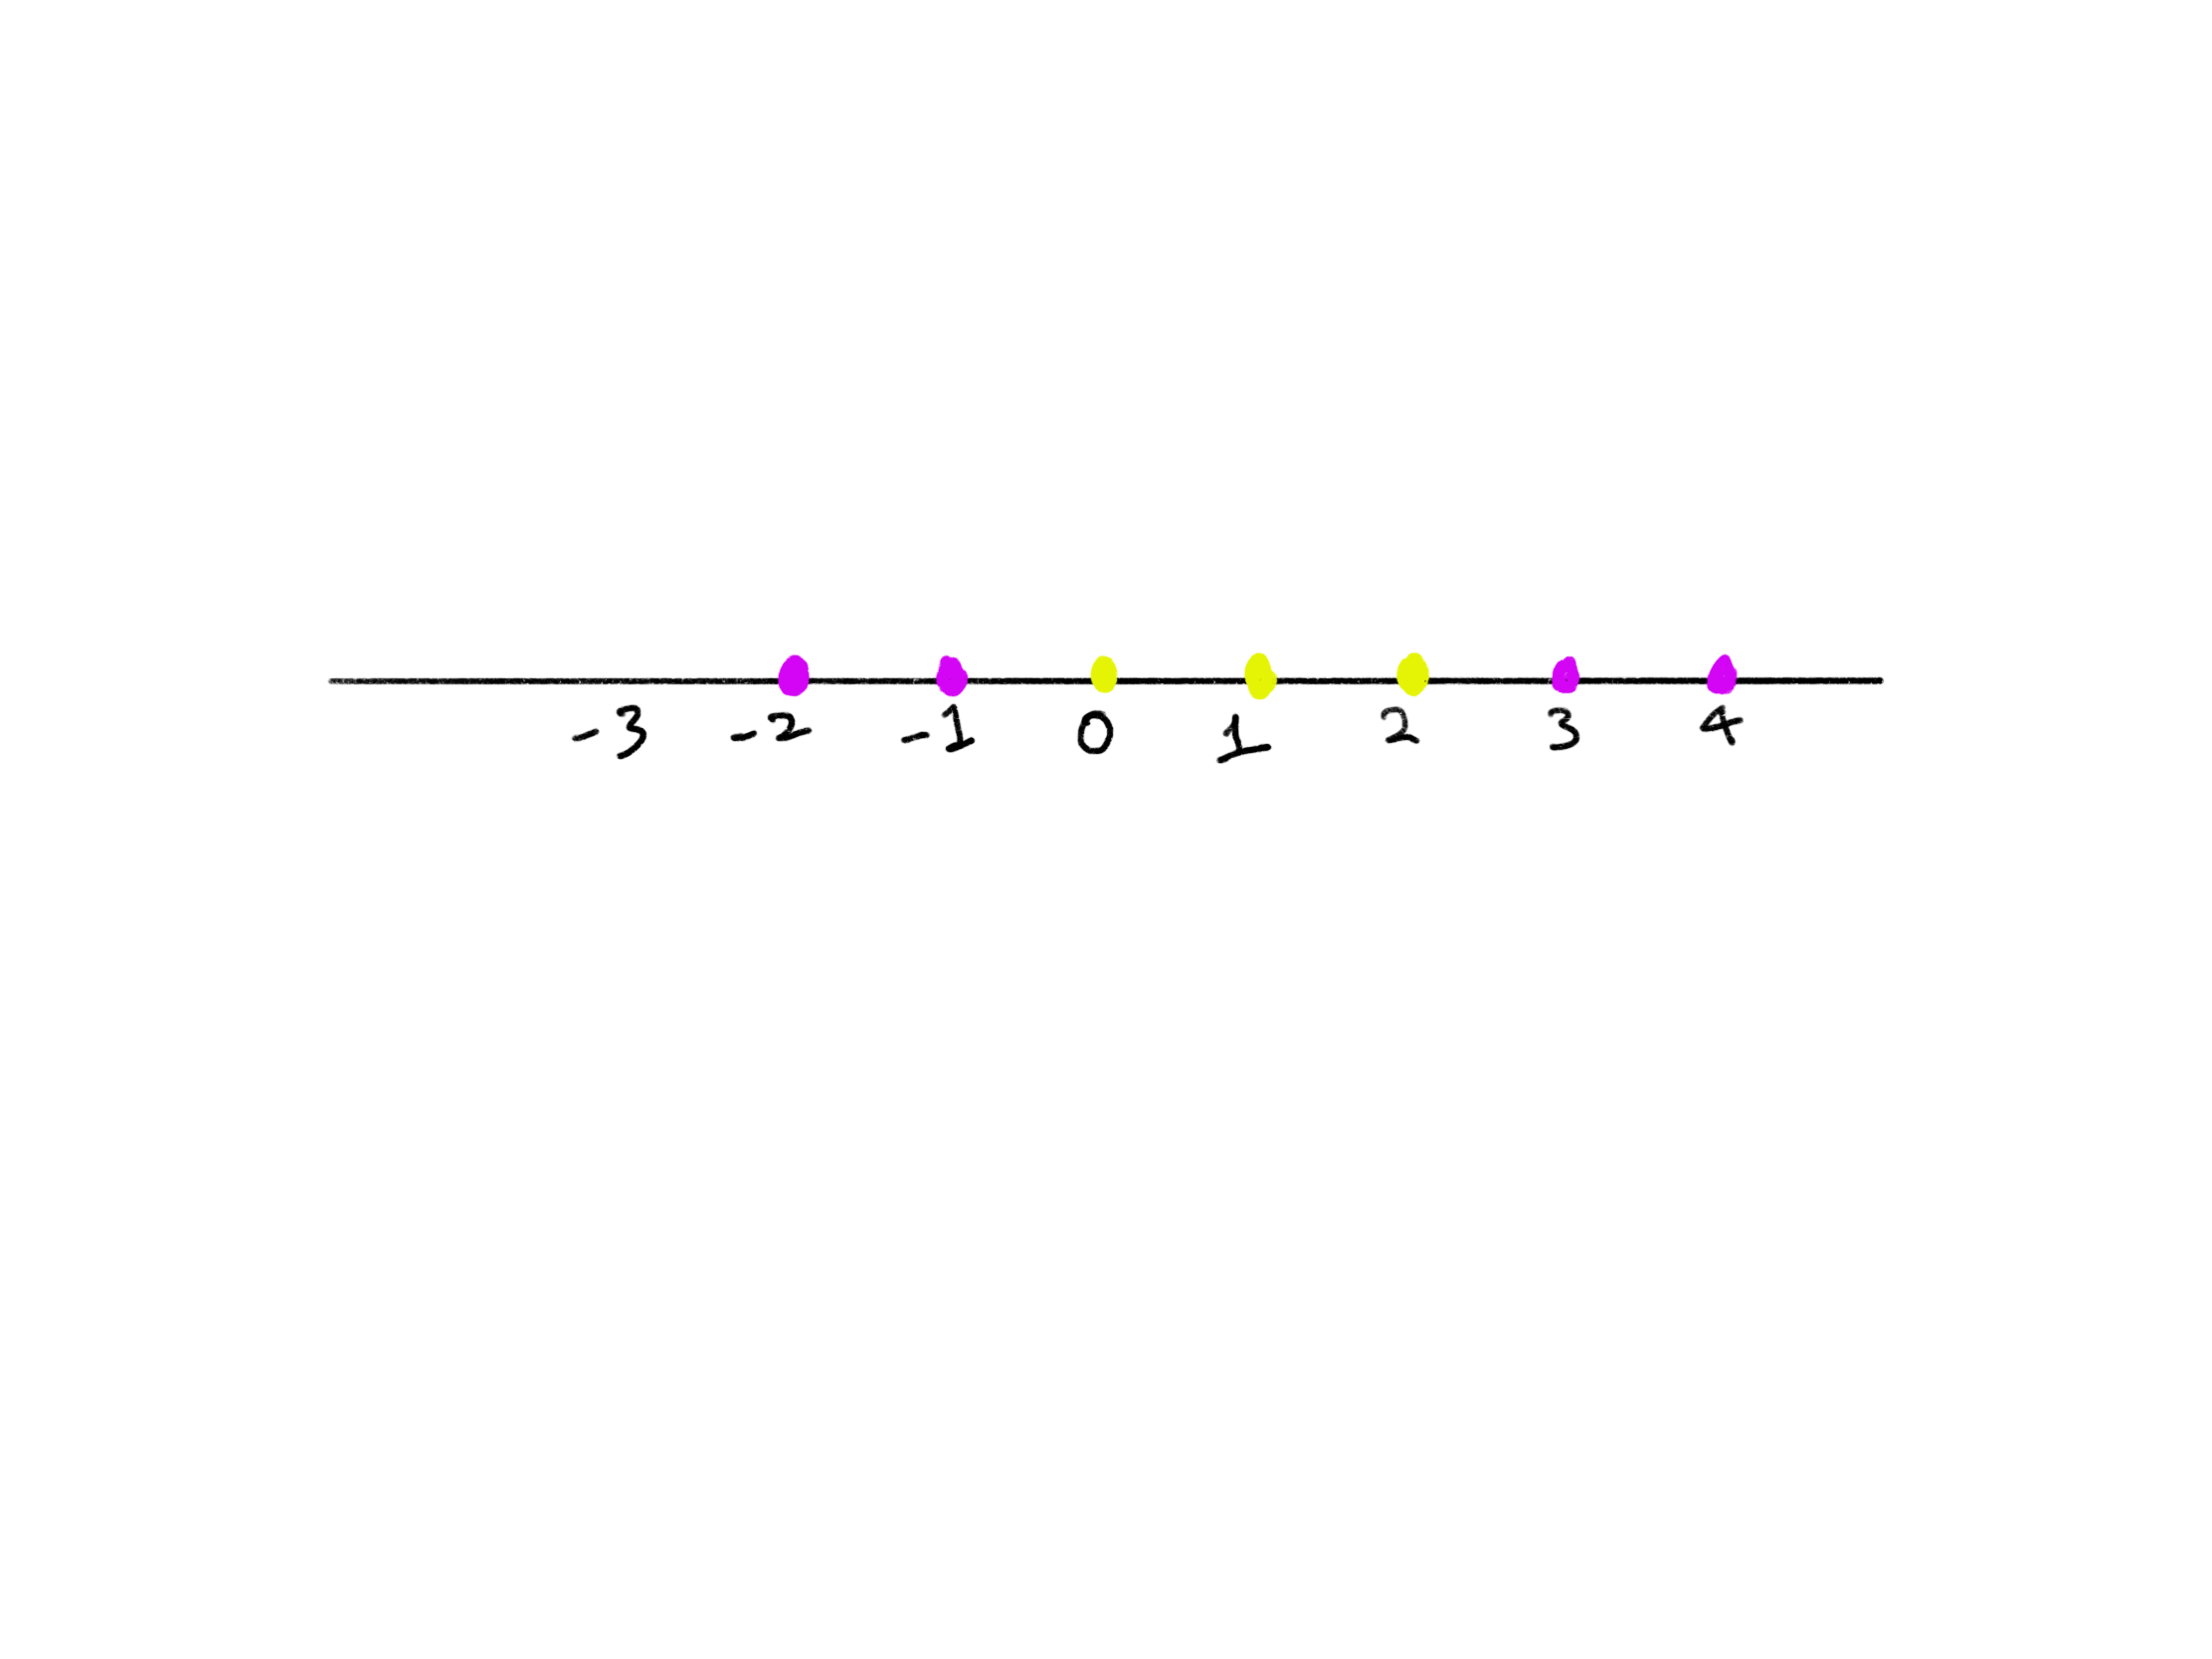
\includegraphics[height=2.5\textwidth]{pik6.png}
      \end{figure}
  \end{minipage} \\
  \vspace{-3cm}
	    $\phi(x) = <\sqrt{2}x, x^{2}>$ \\
	    $K(x_{i}, x_{j}) = (1 + x_{i}x_{j})^{2} - 1$ where $x_{i}x_{j}$ is dot product in lower dimensions \\
	    \begin{align*}
	        (1 + x_{i}x_{j})^{2} - 1 &= 1 + 2x_{i}x_{j} + x_{i}^{2}x_{j}^{2} - 1 \\
	        &= <\sqrt{2}x_{i}, x_{i}^{2}> . <\sqrt{2}x_{j}, x_{j}^{2}>\\
	        &= \phi(x_{i}).\phi(x_{j})
	    \end{align*}
	\end{frame}
	\begin{frame}{Kernel Trick}
	\vspace{-1cm}
	\begin{minipage}{0.3\textwidth}
    % Show the image at item three and afterwards
    
      \begin{figure}
      
        % From https://i.imgur.com/AyzVOIO.jpg
       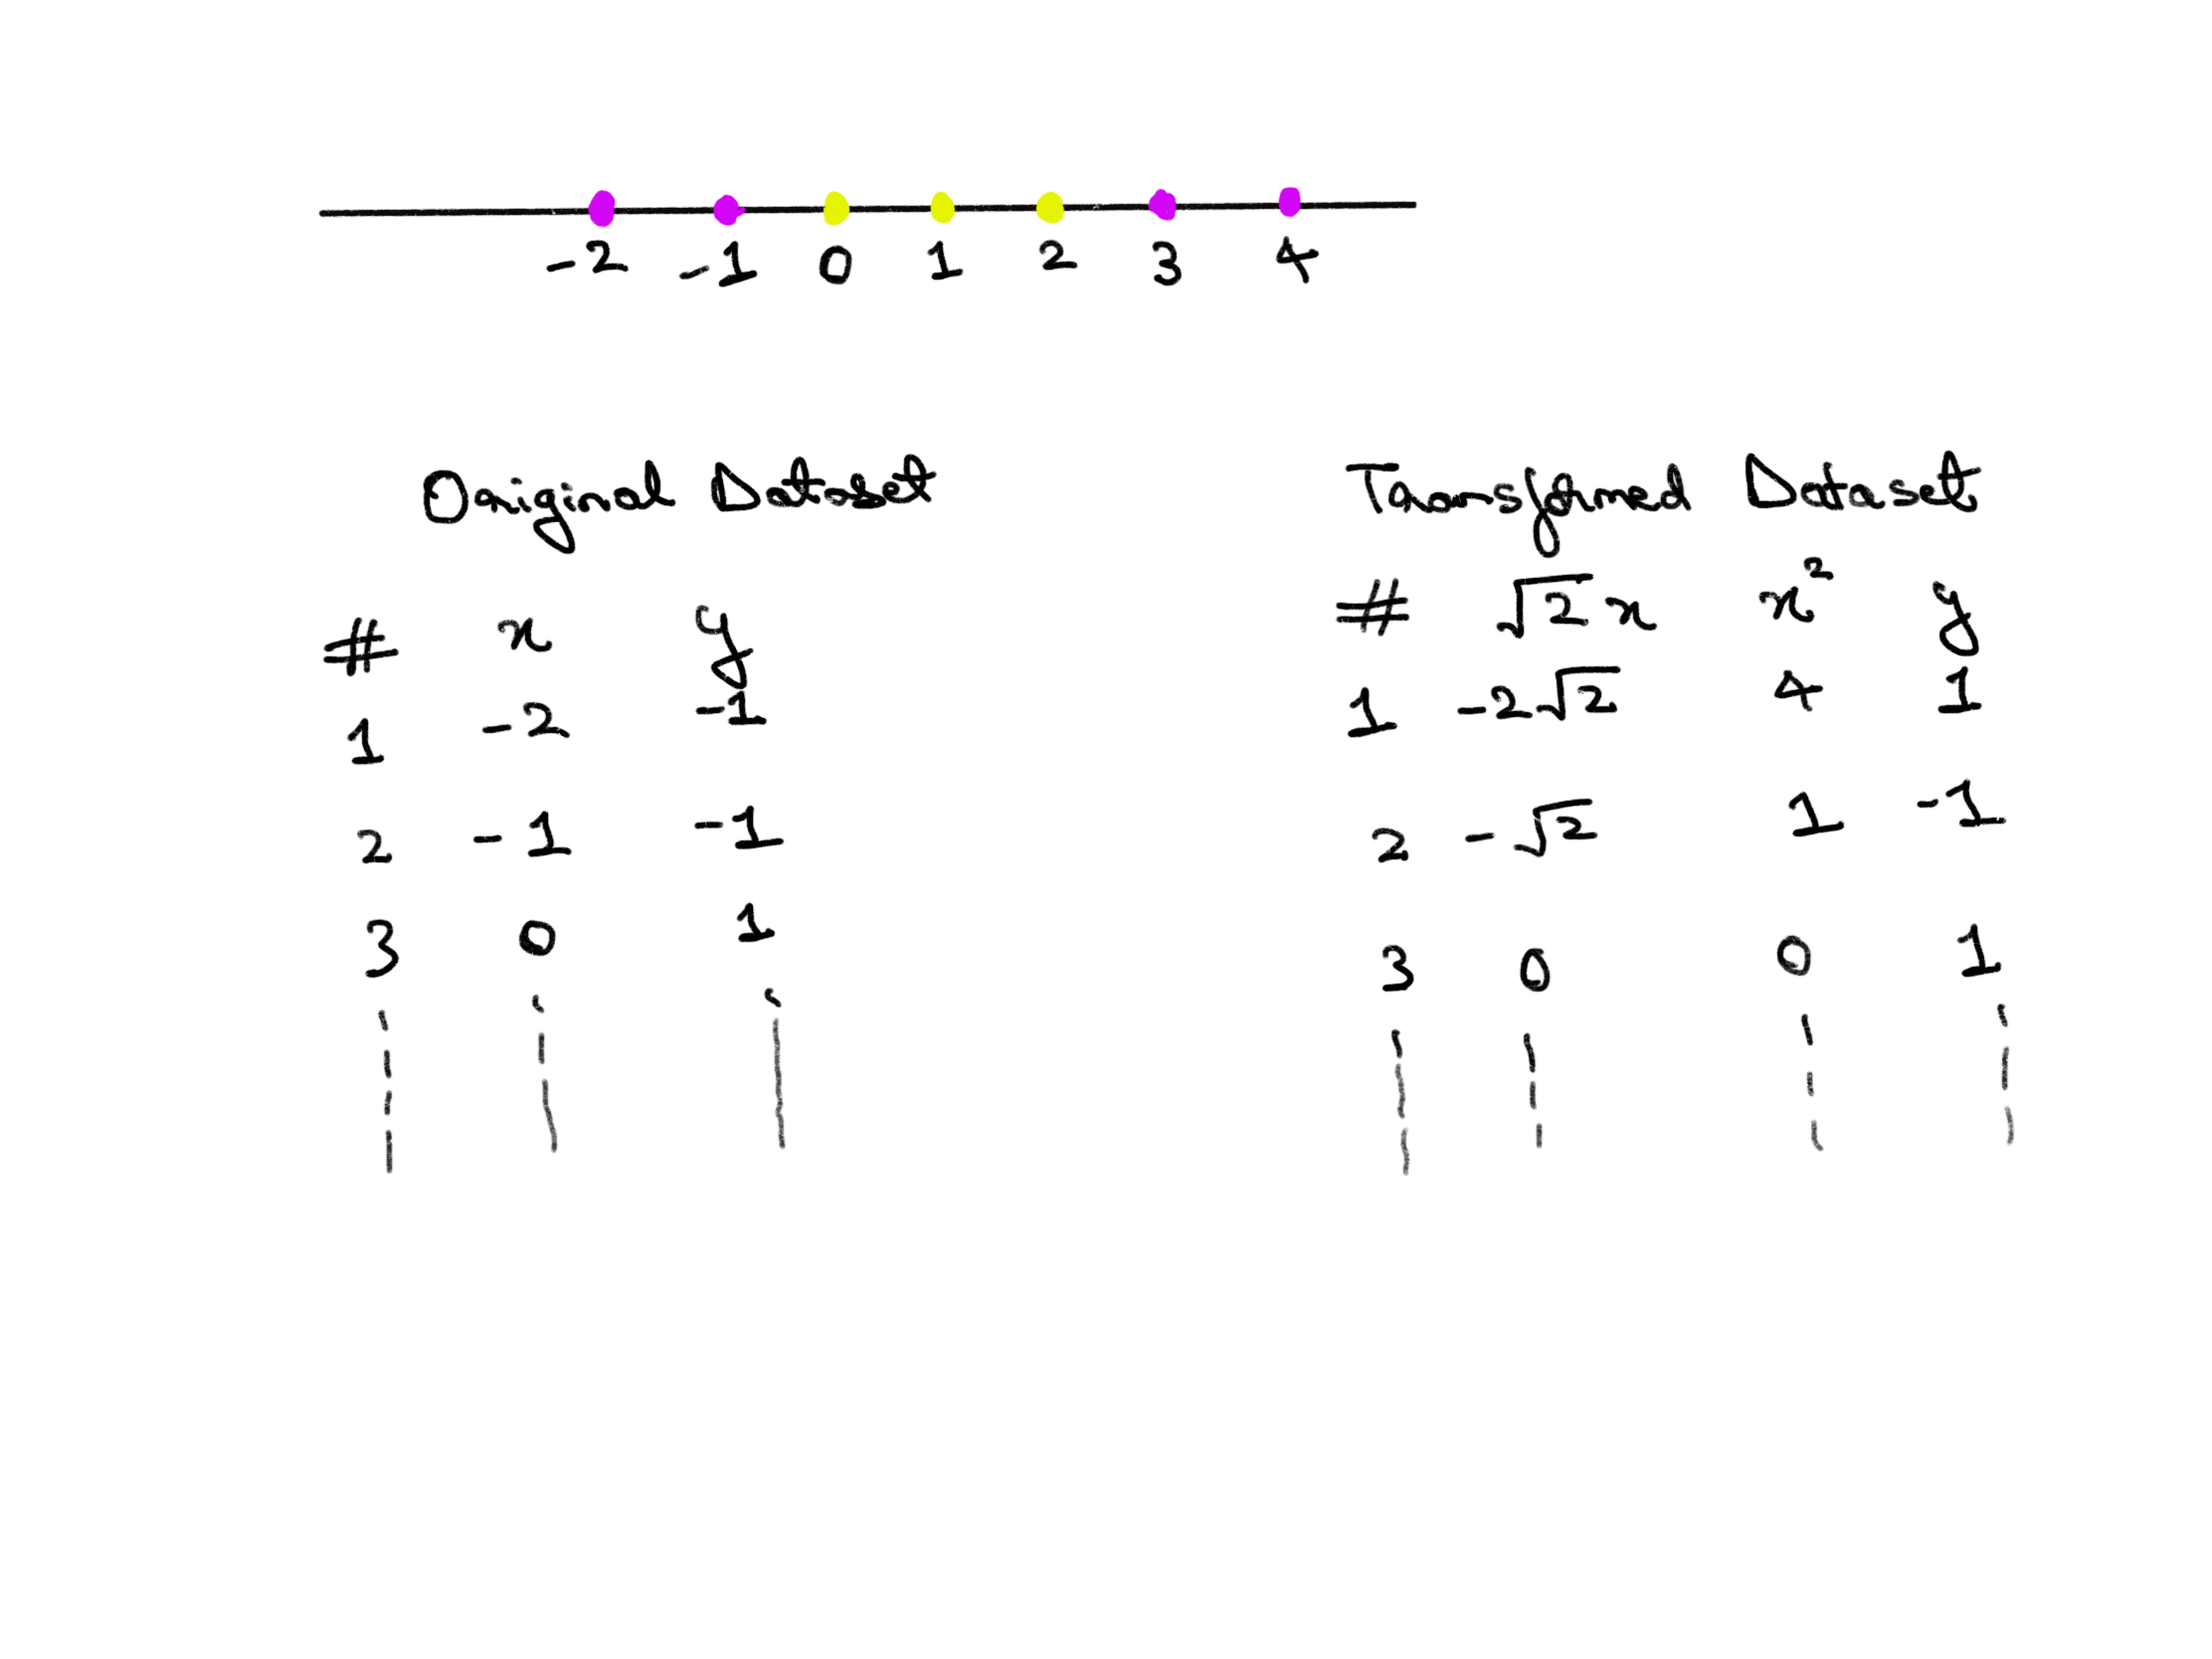
\includegraphics[height=2.5\textwidth]{pik7.png}
      \end{figure}
  \end{minipage} \\
  \vspace{-2cm}
	    $\phi(x_{1}) = <-2\sqrt{2}, 4>; \phi(x_{2}) = <-\sqrt{2}, 1>$ Transformation \\
	    $\phi(x_{1})\phi(x_{2}) = -2\sqrt{2}\times -\sqrt{2} + 4 \times 1 = 8$ Dot product in 2D \\
	    K$(x_{1}, x_{2}) = \{1 + (-2)\times(-1)\}^{2} - 1$ Dot product in 1D
	\end{frame}
	\begin{frame}{Kernel Trick}
	   Q) Why did we use dual form? \\
	   \hspace{0.5cm} Kernels again!! \\
	   \vspace{1cm}
	   Primal form doesn't allow for the kernel trick \\
	   K($\bar{x}_{1}, \bar{x}_{2}$) in dual and compute $\phi(x)$ and then dot product in D dimensions
	\end{frame}
	\begin{frame}{Gram Matrix: (Positive Semi-Definite)}
	$K(x_{i}, x_{j}) = (1 + x_{i}x_{j})^{2}$ \\
	$$
	\begin{matrix}
	& x_{1} & x_{2} & x_{3} & x_{4} & x_{5} & x_{6} & x_{7} \\
	x_{1} & 24 & 8 & 0 & 0 & 8 & 24 & 48 \\
	x_{2} & 8 & 1 & 0 & -1 & 0 & \ldots & \\
	x_{3} & 0 & \ldots & \ldots & \ldots & \ldots & \ldots & \ldots \\
	x_{4} & 0 & & & & & & \\
	x_{5} & 8 & & & & & & \\
	x_{6} & 24 & & & & & & \\
	x_{7} & 48 & & & & & & \\
	\end{matrix}
	$$
	\end{frame}
	\begin{frame}{Another Example}
	\vspace{-1cm}
	\hspace{-2cm}
	\begin{minipage}{0.2\textwidth}
    % Show the image at item three and afterwards
    
      \begin{figure}
      
        % From https://i.imgur.com/AyzVOIO.jpg
       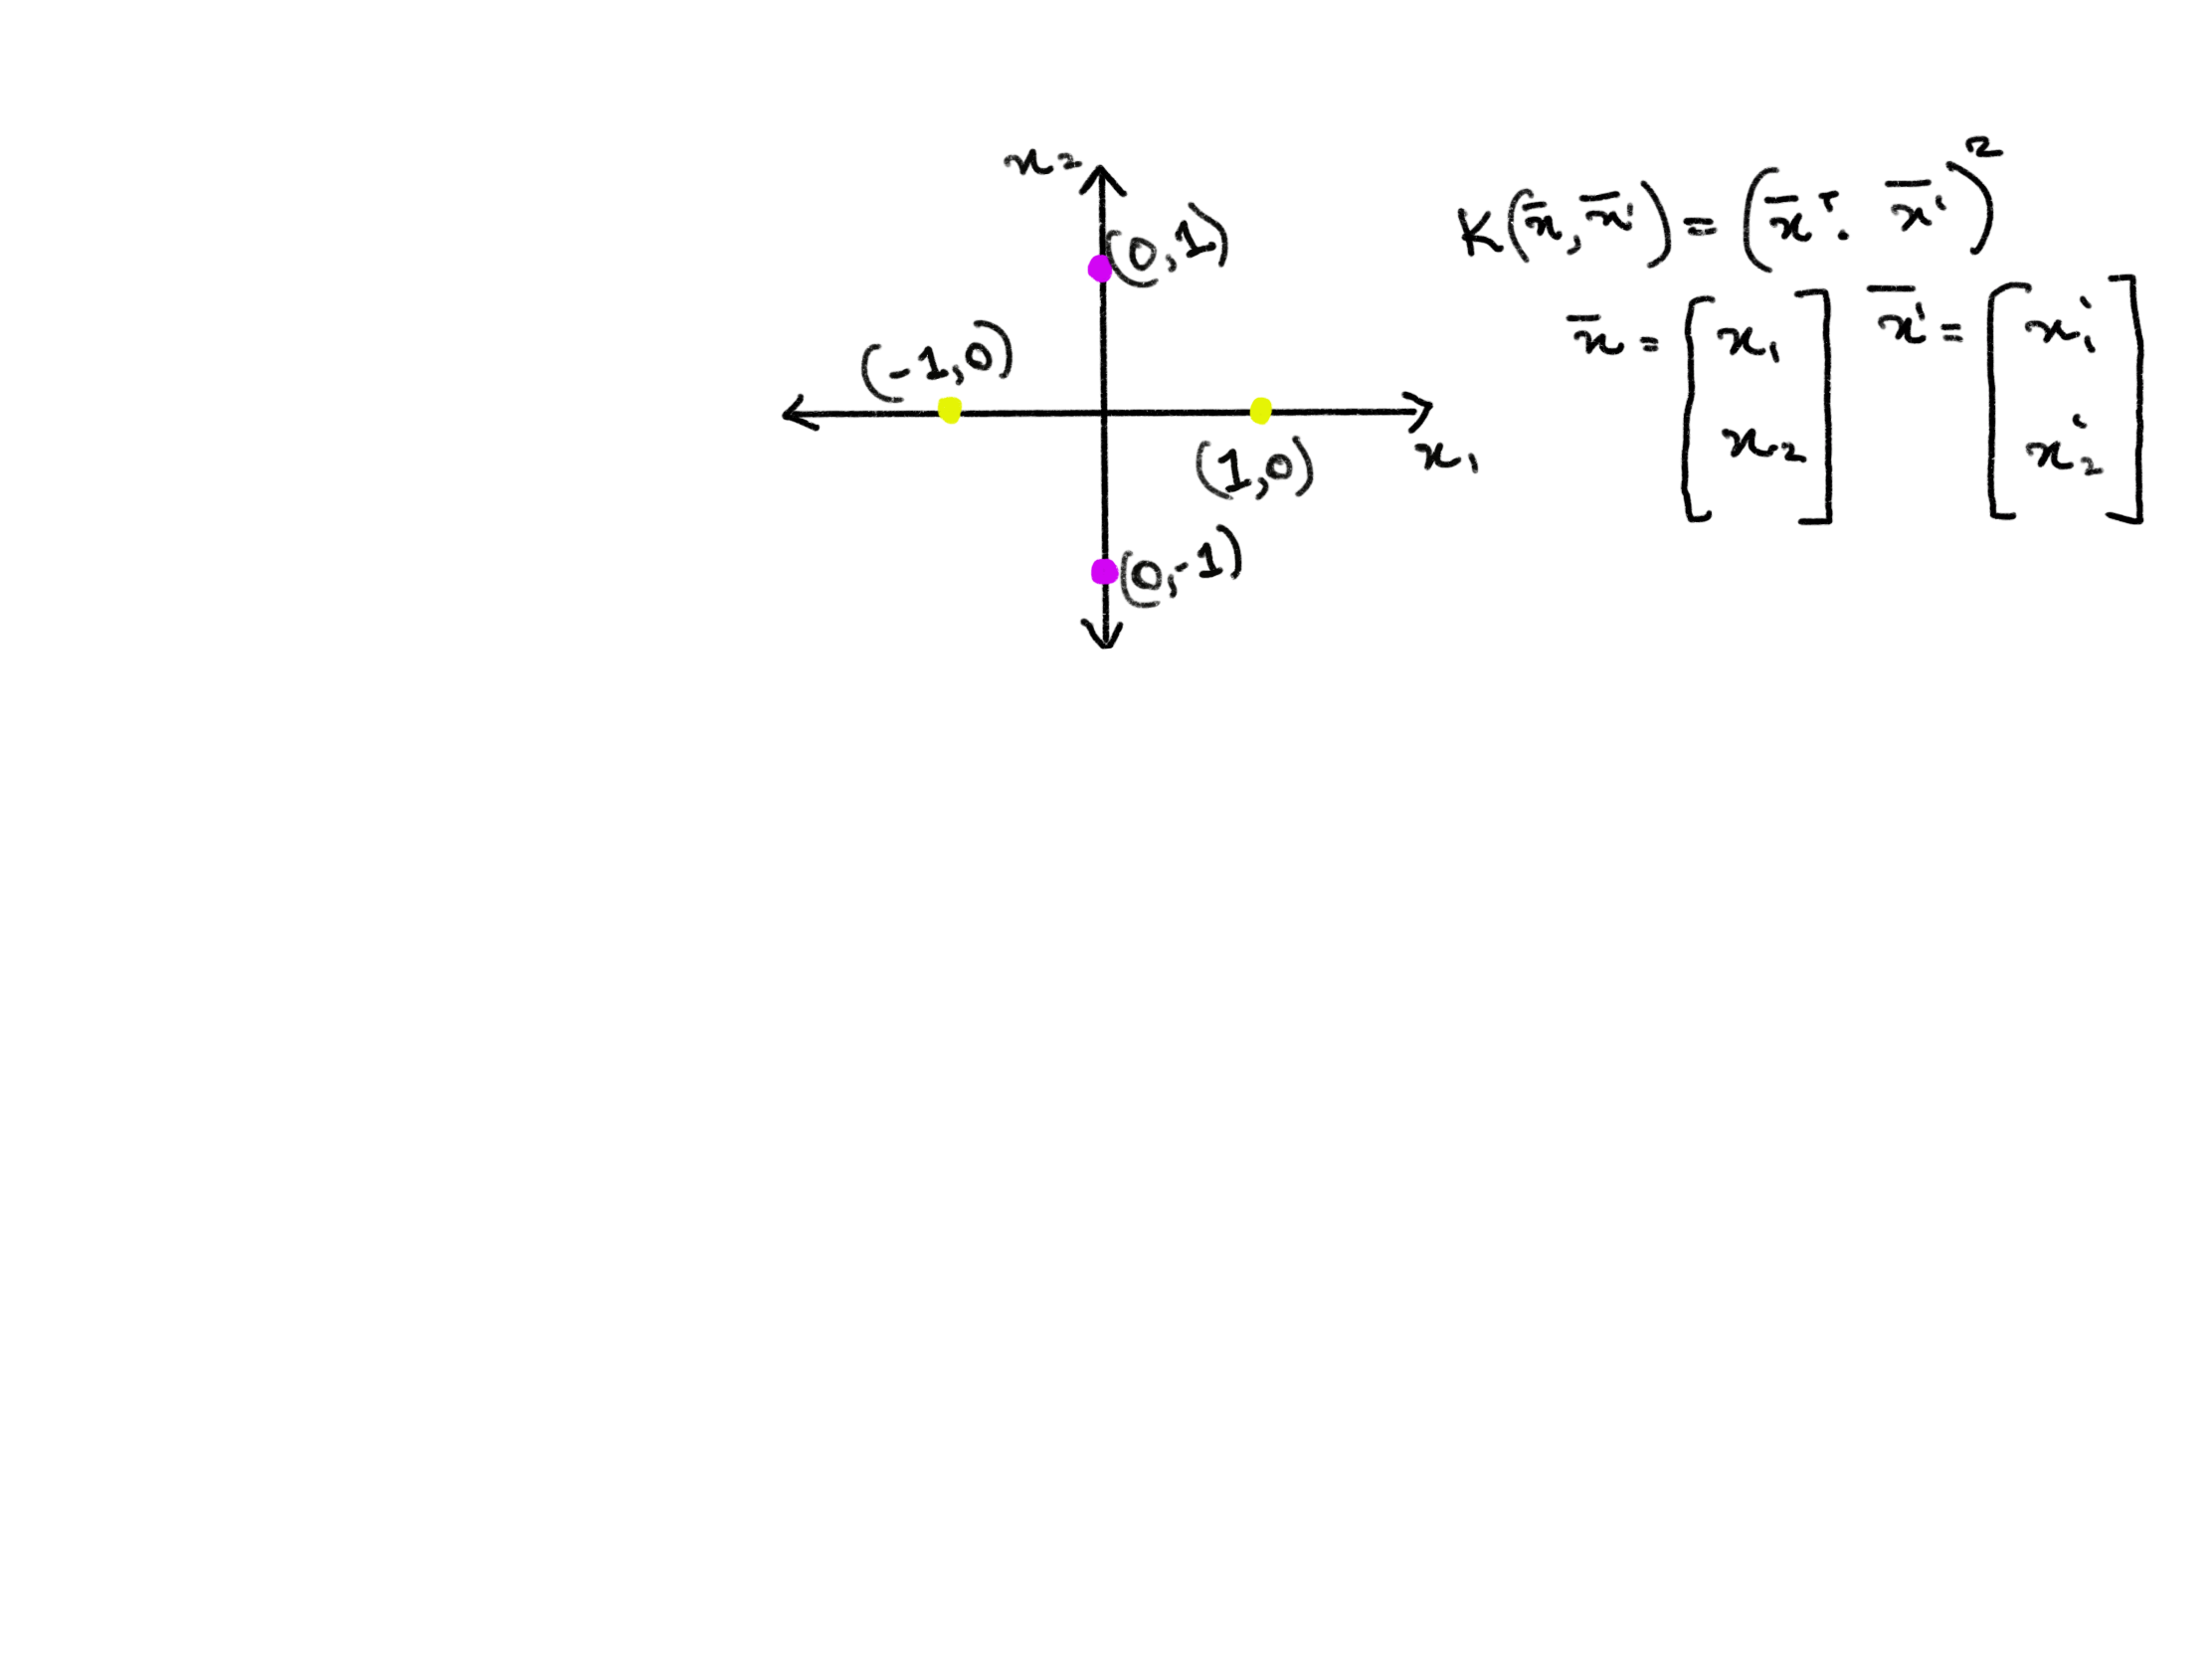
\includegraphics[height=4\textwidth]{pik8.png}
      \end{figure}
  \end{minipage} \\
  \vspace{-5cm}
	    Q) What is $\phi(x)$?
	    \begin{align*}
	        K(\bar{x}, \bar{x'}) &= \phi(\bar{x})\phi(\bar{x'}) \\
	        K(\bar{x}, \bar{x'}) &= \bigg\{\begin{bmatrix}x_{1} & x_{2}\end{bmatrix}\begin{bmatrix}x'_{1} \\ x'_{2}\end{bmatrix}\bigg\}^{2} = (x_{1}x'_{1} + x_{2}x'_{2})^{2} \\
	    \end{align*}
	    \vspace{-1.5cm}
	   $\Longrightarrow \phi(x)=<x_{1}^{2}, \sqrt{2} x_{1} x_{2}, x_{2}^{2}>=x_{1}^{2} x_{1}^{\prime 2}+x_{2}^{2} x_{2}^{\prime 2}+2 x_{1} x_{1}^{\prime} x_{2} x_{2}^{\prime}$
	\end{frame}
	\begin{frame}{Another Example}
	    \begin{figure}
      
        % From https://i.imgur.com/AyzVOIO.jpg
       \hspace{-0.4cm}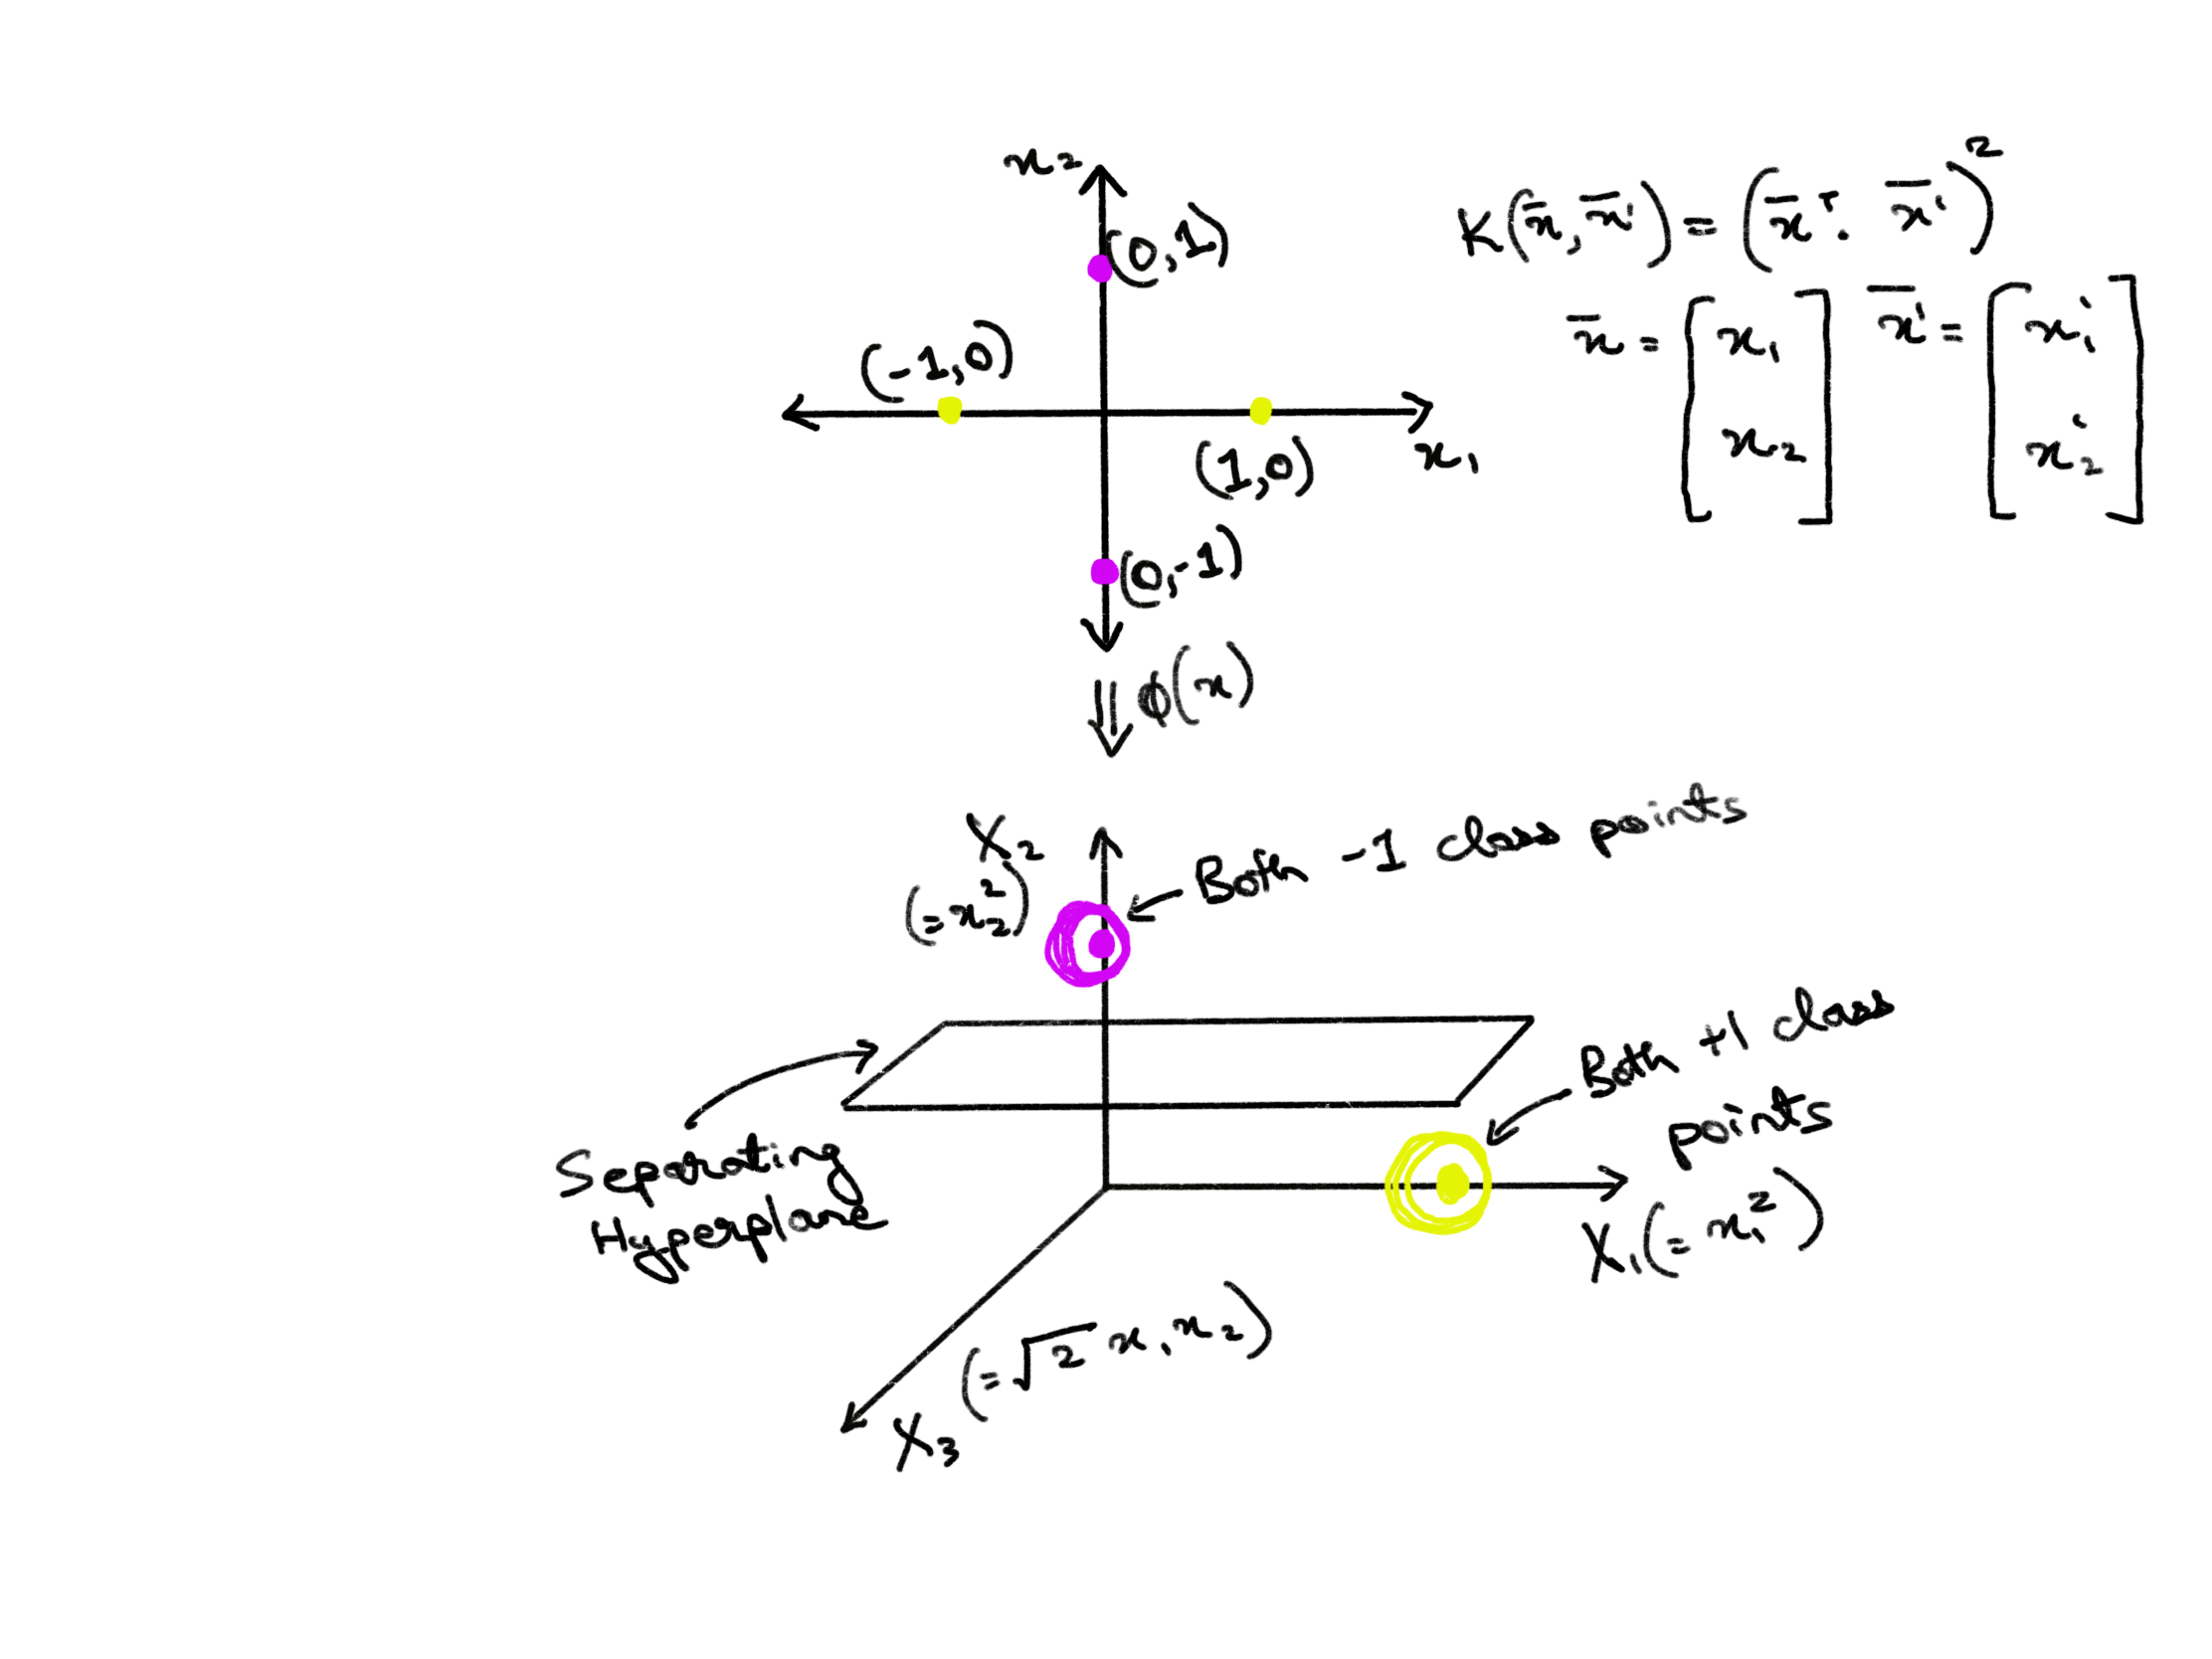
\includegraphics[height=0.75\textwidth]{pik9.png}
      \end{figure}
	\end{frame}
	\begin{frame}{Some Kernels}
	    \begin{enumerate}
	        \item Linear: K($\bar{x}_{1}, \bar{x}_{2}) = \bar{x}_{1}\bar{x}_{2}$
	        \item Polynomial: K($\bar{x}_{1}, \bar{x}_{2}) = (p + \bar{x}_{1}\bar{x}_{2})^{q}$
	        \item Gaussian: K($\bar{x}_{1}, \bar{x}_{2}) = e^{-\gamma\lvert\lvert\bar{x}_{1} - \bar{x}_{2}\rvert\rvert^{2}}$ where $\gamma = \frac{1}{2\sigma^{2}}$ - Also called Radial Basis Function (RBF)
	    \end{enumerate}
	\end{frame}
	\begin{frame}{Kernels}
	    Q) For $\bar{x} = \begin{bmatrix}x_{1} \\ x_{2} \end{bmatrix}$ what space does kernel K($\bar{x}, \bar{x'}) = (1 + \bar{x}\bar{x'})^{3}$ belong to? \\
	    \hspace{0.5cm}
	    $\bar{x} \in \mathbb{R}^{2}$ \\ 
	    \hspace{0.5cm} $\phi(\bar{x}) \in \mathbb{R}^{?}$
	    \begin{align*}
	        K(x, z) &= (1 + x_{1}z_{1} + x_{2}z_{2})^{3} \\
	        &= \ldots \\
	        &= <1, x_{1}, x_{2}, x_{1}^{2}, x_{2}^{2}, x_{1}^{2}x_{2}, x_{1}x_{2}^{2}, x_{1}^{3}, x_{2}^{3}, x_1x_2>
	    \end{align*}
	    \hspace{3cm}10 dimensional?
	\end{frame}
	\begin{frame}{Kernels}
	    Q) For $\bar{x} = x$; what space does RBF kernel lie in? \\
	    \begin{align*}
	        K(x, z) &= e^{-\gamma\lvert\lvert x - z \rvert\rvert^{2}}\\
	        &= e^{-\gamma(x - z)^{2}}
	    \end{align*}
	    Now: $$e^{\alpha} = \sum_{n=0}^{\infty}\frac{\alpha^{n}}{n!}$$
	    
	    $\therefore e^{-\gamma(x - z)^{2}}$ is $\infty$ dimensional!!
	\end{frame}
	\begin{frame}{SVM: Parametric or Non-Parametric}
	    Q) Is SVM parametric or non-parametric? \\
	\end{frame}
	\begin{frame}{SVM: Parametric or Non-Parametric}
	    Q) Is SVM parametric or non-parametric? \\
	    \hspace{0.5cm} Yes and No \\
	    \hspace{0.5cm} Yes $\rightarrow$ Linear kernel or polynomial kernel (form fixed)\\
	    \hspace{0.5cm} No $\rightarrow$ RBF (form changes with data)
	\end{frame}
	\begin{frame}{RBF is Non-Parametric}
	    \begin{align*}
	        \hat{y}(x_{test}) &= sign(\bar{w}\bar{x}_{test} + b) \\
	        &= sign(\sum_{j=1}^{N_{SV}}\alpha_{j}y_{j}\bar{x}_{j}\bar{x}_{test} + b)\\
	        \hat{y}(X_{test}) &= sign(\sum_{j=1}^{N}\alpha_{j}y_{j} K(\bar{x}_{j}, \bar{x}_{test}) + b)
	    \end{align*}
	    $\alpha_{j} = 0$ where $j \neq$ S.V.
	\end{frame}
	\begin{frame}{RBF is Non-Parametric}
	    Now K($\bar{x}_{j}, \bar{x}_{test}$) for RBF is:
	    $$e^{-\gamma \lvert\lvert\bar{x}_{j} - \bar{x}_{test}\rvert\rvert^{2}}$$
	    
	    $\therefore$ Hypothesis is a function of ``all'' train points \\
	    Closer $\bar{x}$ is to $\bar{x}_{N}$; more is it influencing $\hat{y}(\bar{x})$ - hypothesis function
	    \vspace{-4cm}
	    \begin{minipage}{0.2\textwidth}
    % Show the image at item three and afterwards
    \vspace{-2cm}
      \begin{figure}
      
        % From https://i.imgur.com/AyzVOIO.jpg
       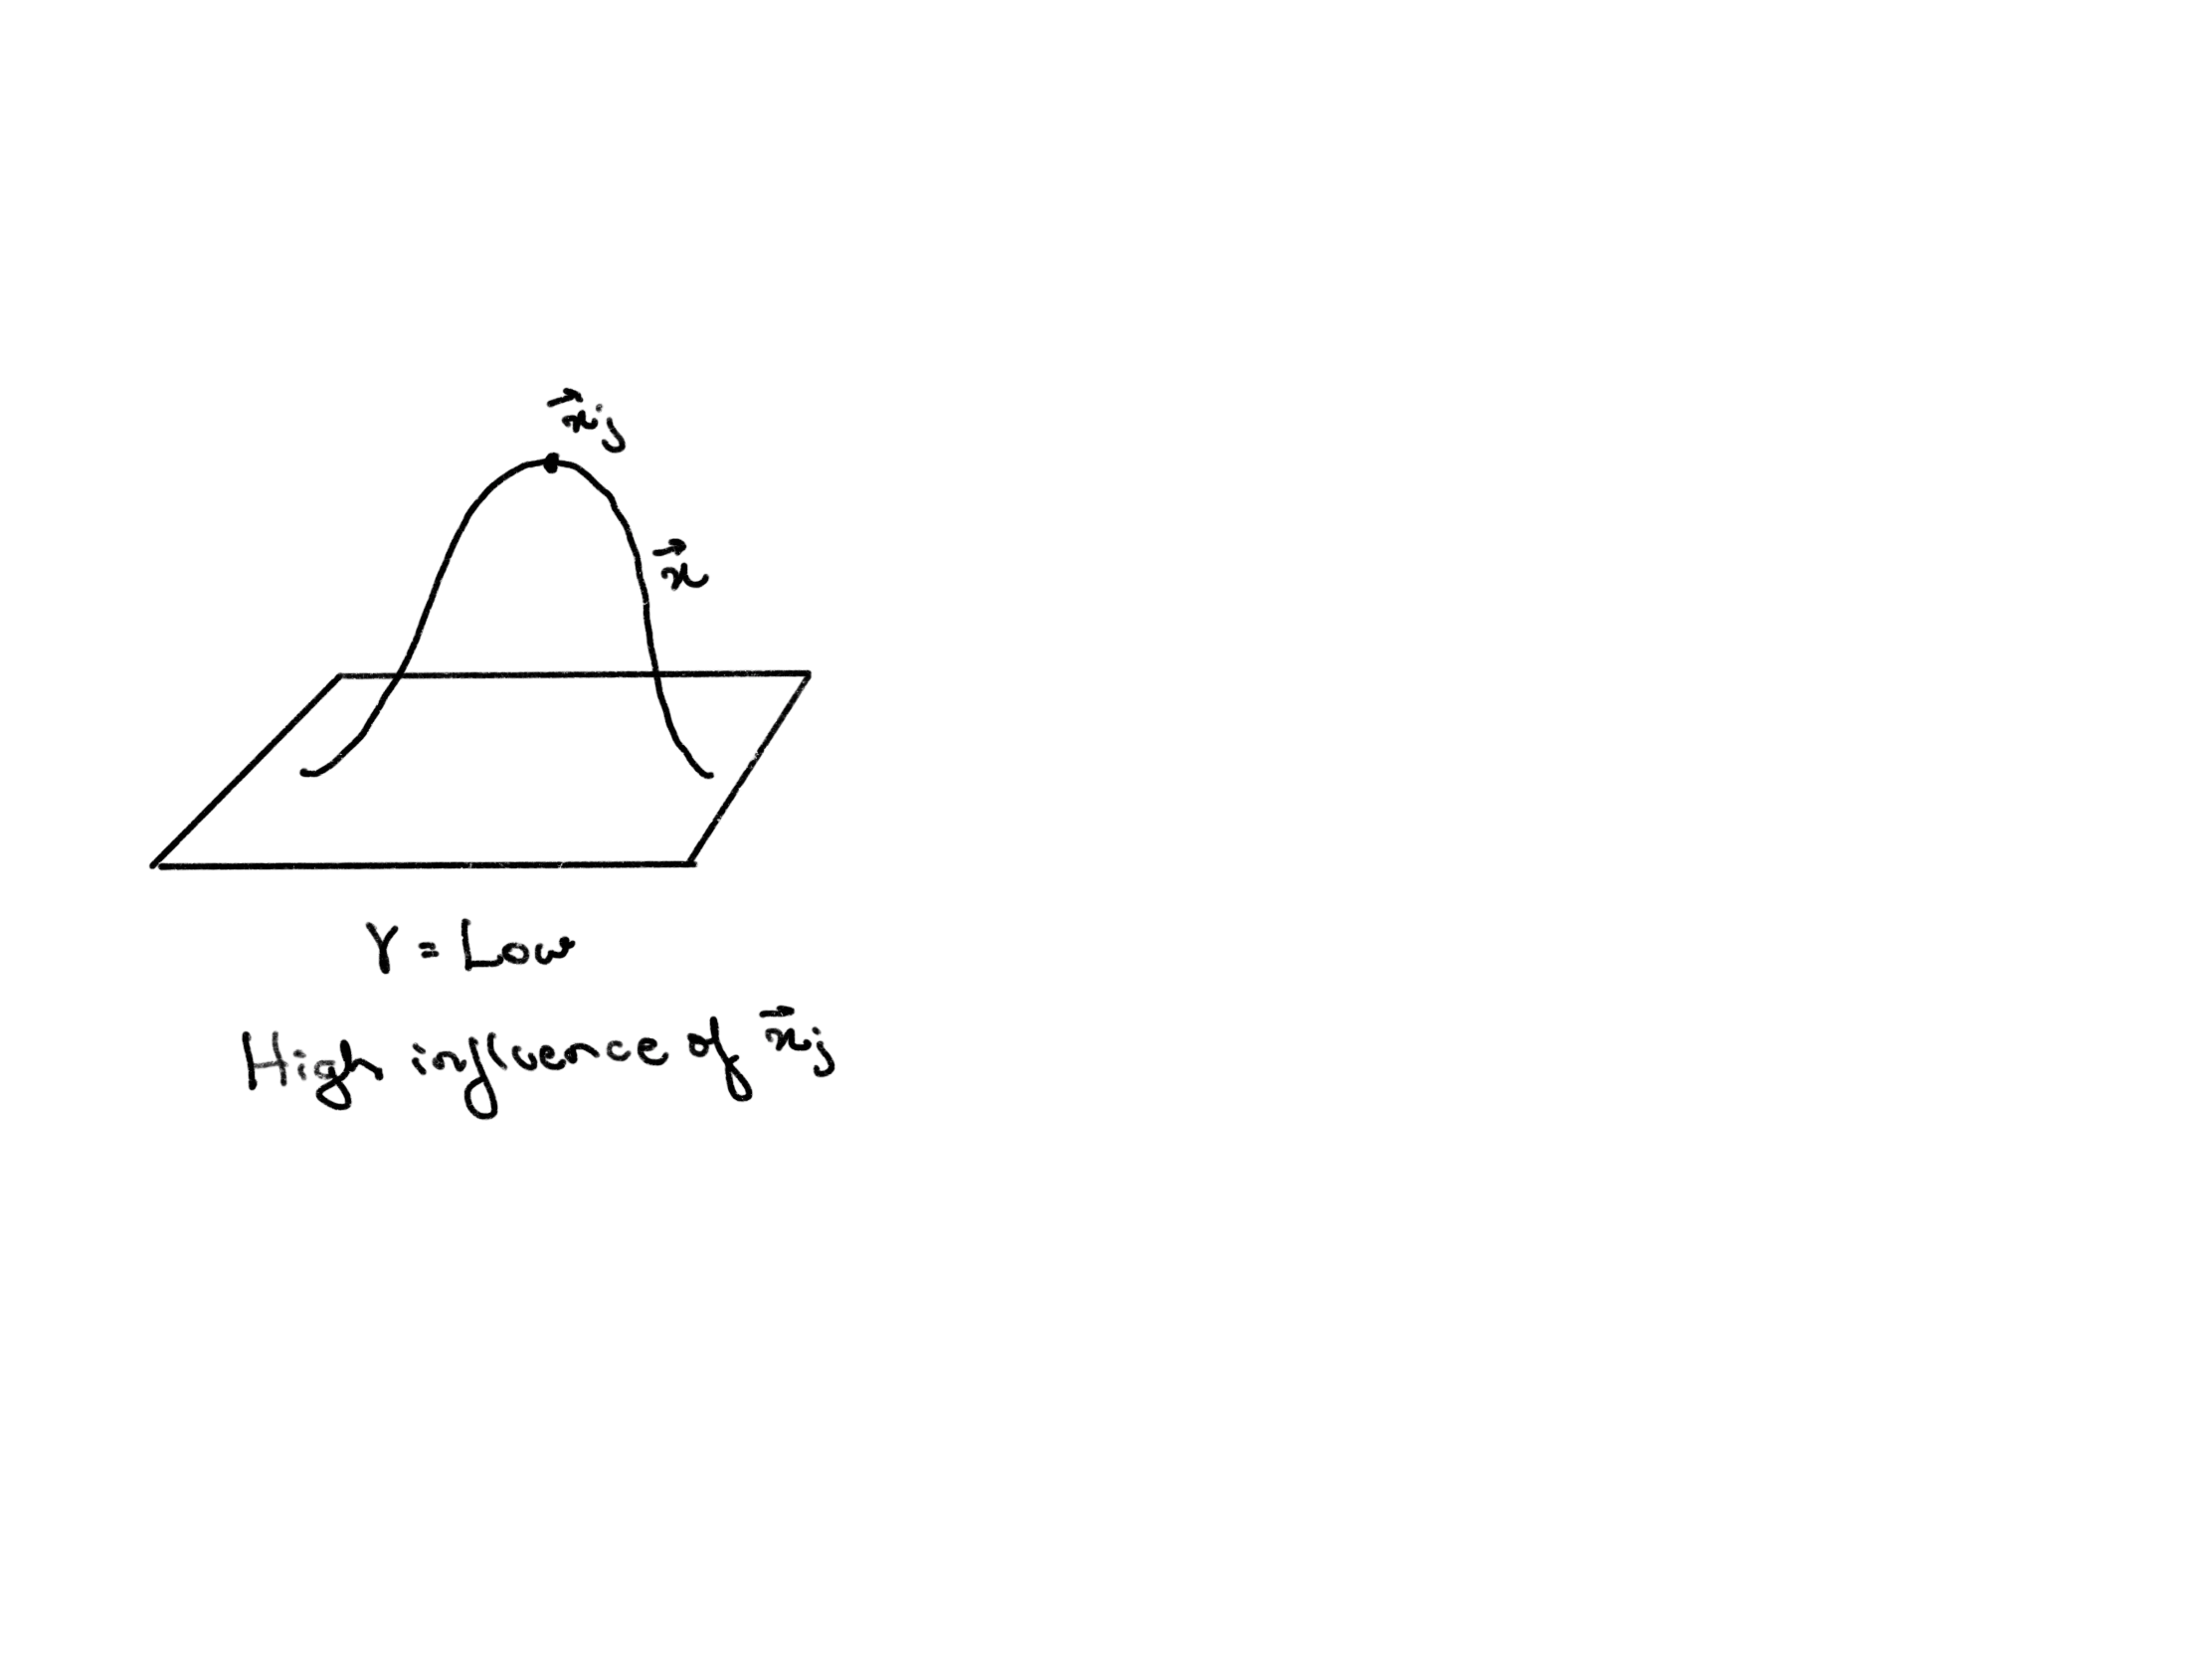
\includegraphics[height=4\textwidth]{pik10.png}
      \end{figure}
  \end{minipage} \\
	\end{frame}
	\begin{frame}{RBF is Non-Parametric}
		\begin{itemize}[<+->]
			\item Now if we add a point to the dataset 
			\item Functional form can adapt (similar to KNN) 
			\item $\therefore$ SVM with RBF kernel is non-parametric
		\end{itemize}
	\end{frame}

	\begin{frame}{Interpretation of RBF}
		\begin{itemize}[<+->]
			\item $\hat{y}(x) = sign(\sum \alpha_{i}y_{i}e^{-\lvert\lvert x - x_{i} \rvert\rvert^{2}} + b)$
			\item ${-\lvert\lvert x - x_{i} \rvert\rvert^{2}}$ corresponds to radial term
			\item $\sum \alpha_{i}y_{i}$ is the activation component
			\item $e^{-\lvert\lvert x - x_{i} \rvert\rvert^{2}}$ is the basis component
		\end{itemize}
	    
	    
	\end{frame}
	\begin{frame}{RBF: Effect of $\gamma$}
	\vspace{2cm}
	    $\gamma$: How far is the influence of a single training sample \\
	    \vspace{-2cm}
	    \begin{minipage}{0.2\textwidth}
    % Show the image at item three and afterwards
      \begin{figure}
      
        % From https://i.imgur.com/AyzVOIO.jpg
       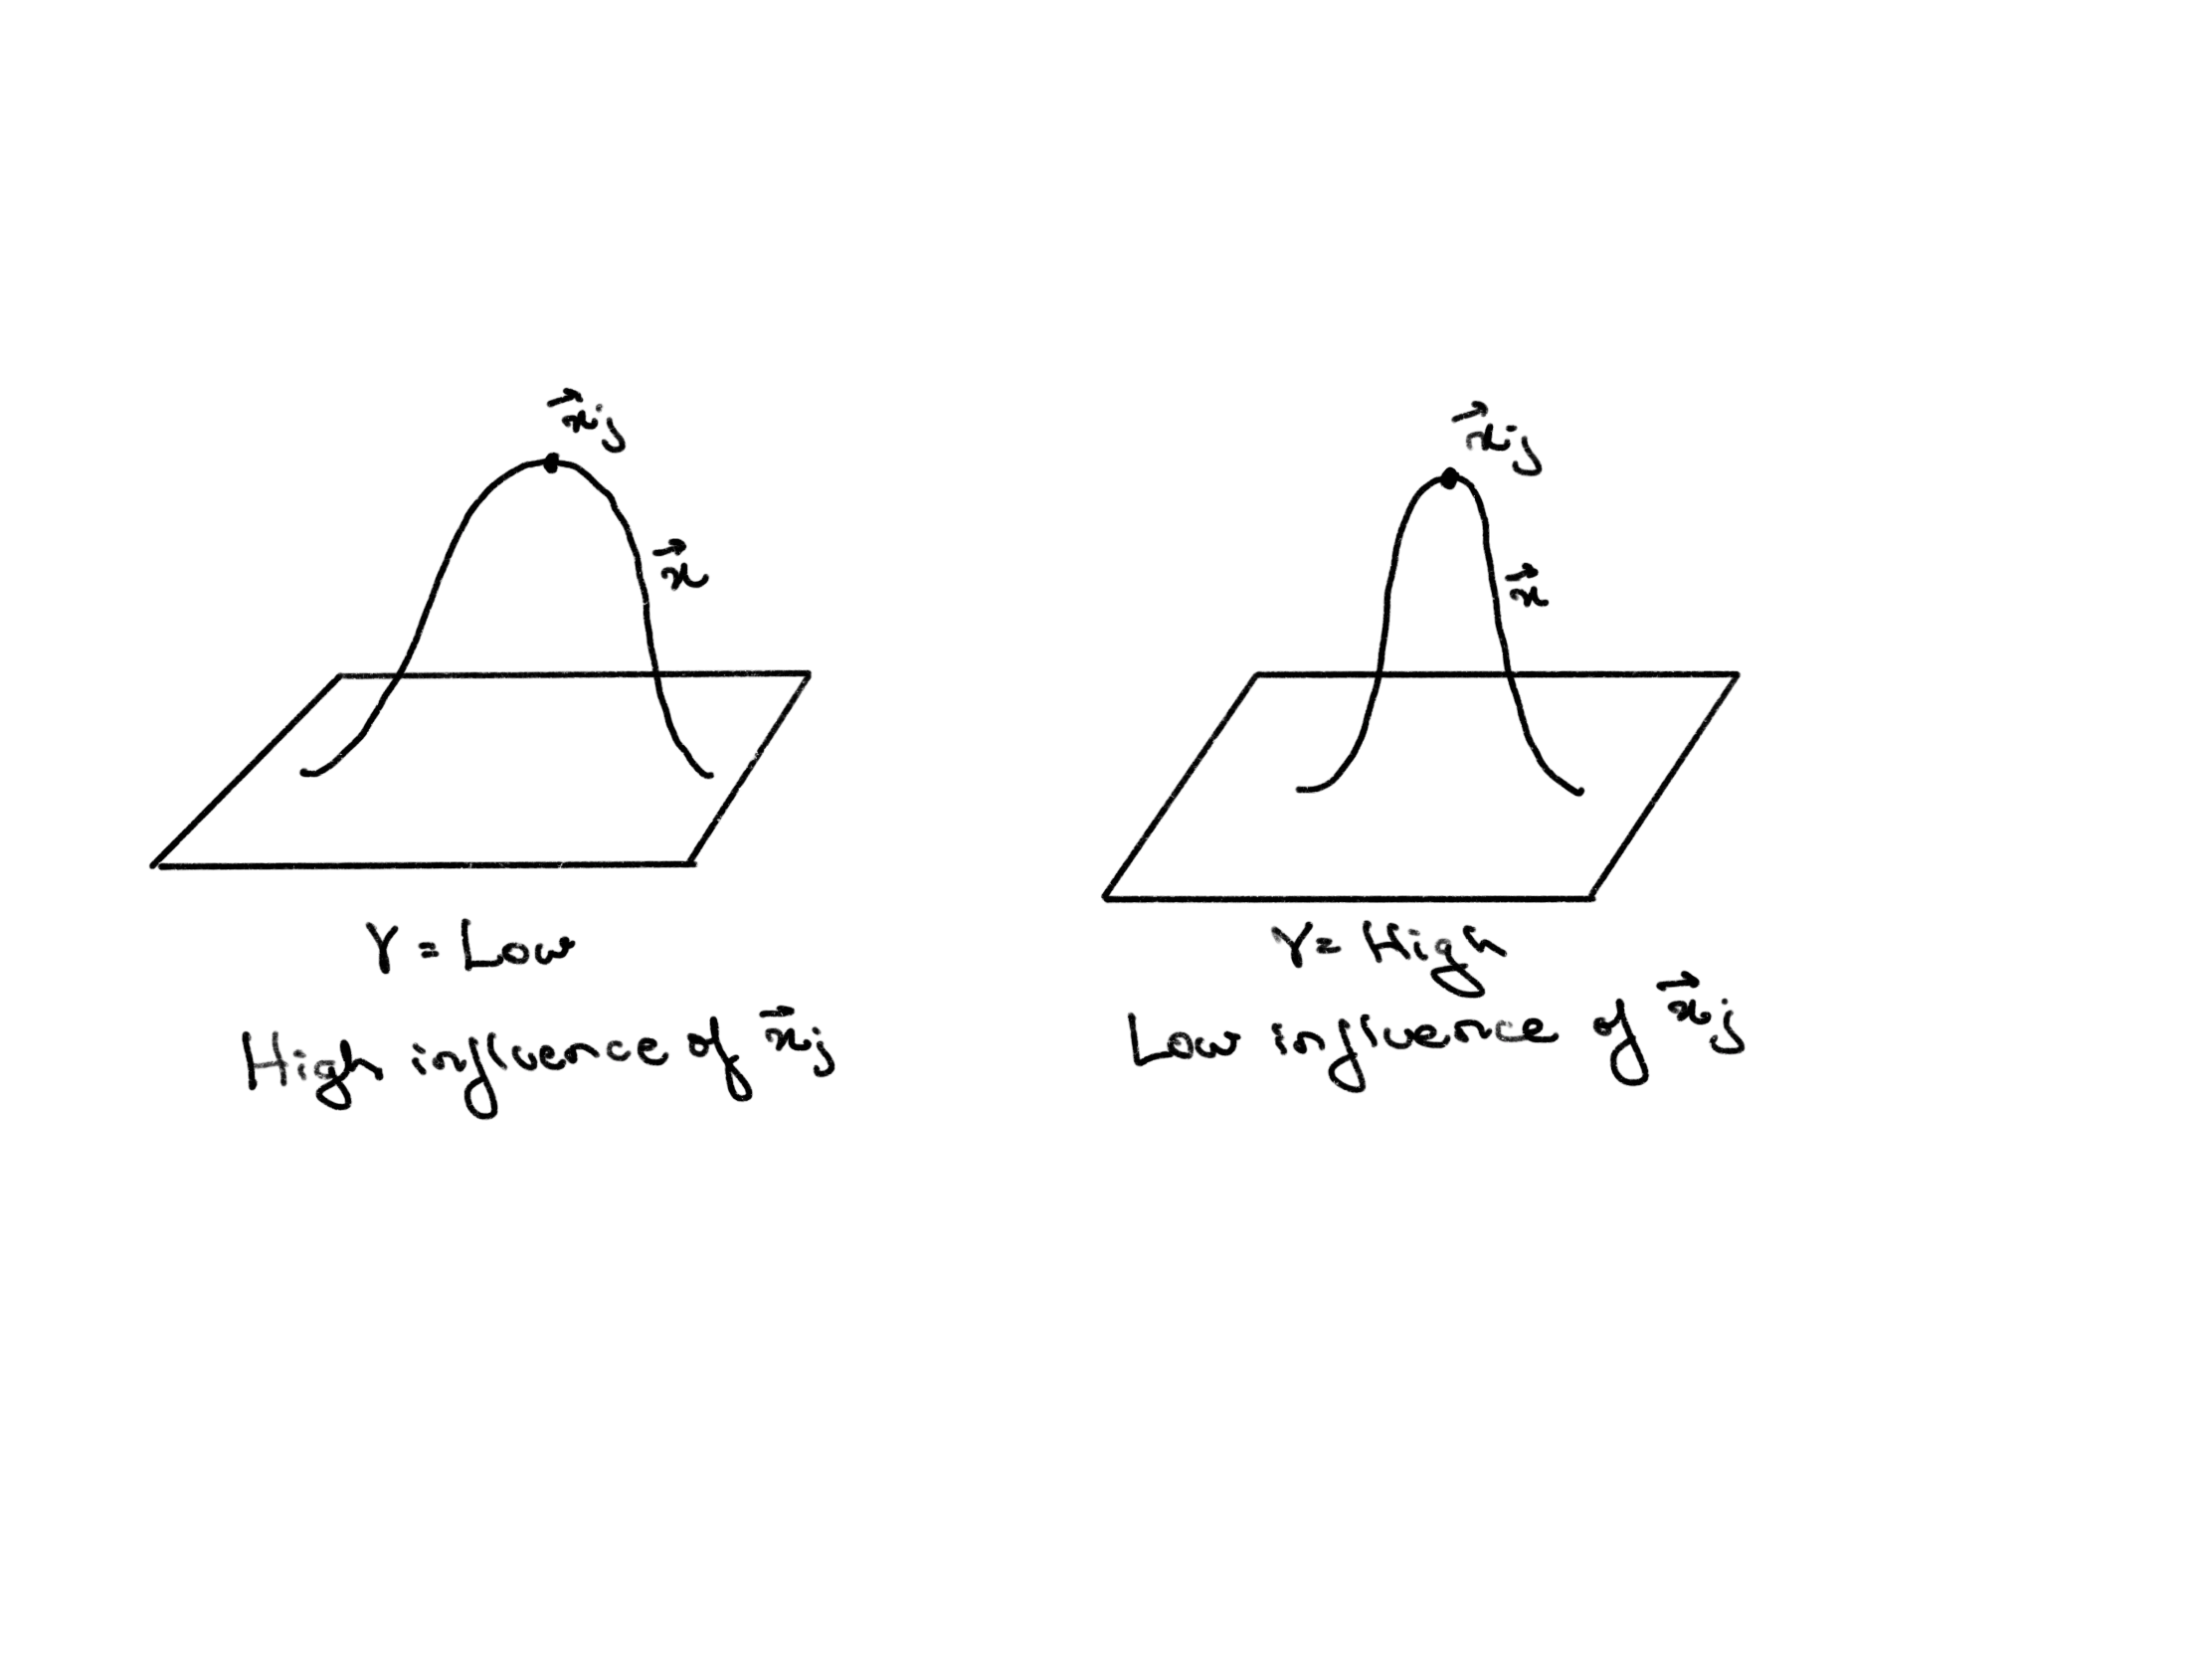
\includegraphics[height=4\textwidth]{pik11.png}
      \end{figure}
  \end{minipage} \\
	\end{frame}

	
\end{document}
